\documentclass[twoside]{book}

% Packages required by doxygen
\usepackage{fixltx2e}
\usepackage{calc}
\usepackage{doxygen}
\usepackage[export]{adjustbox} % also loads graphicx
\usepackage{graphicx}
\usepackage[utf8]{inputenc}
\usepackage{makeidx}
\usepackage{multicol}
\usepackage{multirow}
\PassOptionsToPackage{warn}{textcomp}
\usepackage{textcomp}
\usepackage[nointegrals]{wasysym}
\usepackage[table]{xcolor}

% Font selection
\usepackage[T1]{fontenc}
\usepackage[scaled=.90]{helvet}
\usepackage{courier}
\usepackage{amssymb}
\usepackage{sectsty}
\renewcommand{\familydefault}{\sfdefault}
\allsectionsfont{%
  \fontseries{bc}\selectfont%
  \color{darkgray}%
}
\renewcommand{\DoxyLabelFont}{%
  \fontseries{bc}\selectfont%
  \color{darkgray}%
}
\newcommand{\+}{\discretionary{\mbox{\scriptsize$\hookleftarrow$}}{}{}}

% Page & text layout
\usepackage{geometry}
\geometry{%
  a4paper,%
  top=2.5cm,%
  bottom=2.5cm,%
  left=2.5cm,%
  right=2.5cm%
}
\tolerance=750
\hfuzz=15pt
\hbadness=750
\setlength{\emergencystretch}{15pt}
\setlength{\parindent}{0cm}
\setlength{\parskip}{0.2cm}
\makeatletter
\renewcommand{\paragraph}{%
  \@startsection{paragraph}{4}{0ex}{-1.0ex}{1.0ex}{%
    \normalfont\normalsize\bfseries\SS@parafont%
  }%
}
\renewcommand{\subparagraph}{%
  \@startsection{subparagraph}{5}{0ex}{-1.0ex}{1.0ex}{%
    \normalfont\normalsize\bfseries\SS@subparafont%
  }%
}
\makeatother

% Headers & footers
\usepackage{fancyhdr}
\pagestyle{fancyplain}
\fancyhead[LE]{\fancyplain{}{\bfseries\thepage}}
\fancyhead[CE]{\fancyplain{}{}}
\fancyhead[RE]{\fancyplain{}{\bfseries\leftmark}}
\fancyhead[LO]{\fancyplain{}{\bfseries\rightmark}}
\fancyhead[CO]{\fancyplain{}{}}
\fancyhead[RO]{\fancyplain{}{\bfseries\thepage}}
\fancyfoot[LE]{\fancyplain{}{}}
\fancyfoot[CE]{\fancyplain{}{}}
\fancyfoot[RE]{\fancyplain{}{\bfseries\scriptsize Generated on Mon Feb 9 2015 23\+:42\+:56 for mitgcm by Doxygen }}
\fancyfoot[LO]{\fancyplain{}{\bfseries\scriptsize Generated on Mon Feb 9 2015 23\+:42\+:56 for mitgcm by Doxygen }}
\fancyfoot[CO]{\fancyplain{}{}}
\fancyfoot[RO]{\fancyplain{}{}}
\renewcommand{\footrulewidth}{0.4pt}
\renewcommand{\chaptermark}[1]{%
  \markboth{#1}{}%
}
\renewcommand{\sectionmark}[1]{%
  \markright{\thesection\ #1}%
}

% Indices & bibliography
\usepackage{natbib}
\usepackage[titles]{tocloft}
\setcounter{tocdepth}{3}
\setcounter{secnumdepth}{5}
\makeindex

% Hyperlinks (required, but should be loaded last)
\usepackage{ifpdf}
\ifpdf
  \usepackage[pdftex,pagebackref=true]{hyperref}
\else
  \usepackage[ps2pdf,pagebackref=true]{hyperref}
\fi
\hypersetup{%
  colorlinks=true,%
  linkcolor=blue,%
  citecolor=blue,%
  unicode%
}

% Custom commands
\newcommand{\clearemptydoublepage}{%
  \newpage{\pagestyle{empty}\cleardoublepage}%
}


%===== C O N T E N T S =====

\begin{document}

% Titlepage & ToC
\hypersetup{pageanchor=false,
             bookmarks=true,
             bookmarksnumbered=true,
             pdfencoding=unicode
            }
\pagenumbering{roman}
\begin{titlepage}
\vspace*{7cm}
\begin{center}%
{\Large mitgcm }\\
\vspace*{1cm}
{\large Generated by Doxygen 1.8.9.1}\\
\vspace*{0.5cm}
{\small Mon Feb 9 2015 23:42:56}\\
\end{center}
\end{titlepage}
\clearemptydoublepage
\tableofcontents
\clearemptydoublepage
\pagenumbering{arabic}
\hypersetup{pageanchor=true}

%--- Begin generated contents ---
\chapter{Documentation for python package mitgcm}
\label{index}\hypertarget{index}{}\begin{DoxyAuthor}{Author}
Ed Doddridge
\end{DoxyAuthor}
\hypertarget{index_Overview}{}\section{Overview}\label{index_Overview}
This package provides methods and classes for analysing the output of mitgcm simulations.\hypertarget{index_Revision}{}\section{History}\label{index_Revision}
January 2015\+: Added documentation

February 2015\+: Added streamline and streakline algorithms 
\chapter{Namespace Index}
\section{Namespace List}
Here is a list of all namespaces with brief descriptions\+:\begin{DoxyCompactList}
\item\contentsline{section}{\hyperlink{namespacemitgcm}{mitgcm} }{\pageref{namespacemitgcm}}{}
\item\contentsline{section}{\hyperlink{namespacemitgcm_1_1core}{mitgcm.\+core} }{\pageref{namespacemitgcm_1_1core}}{}
\item\contentsline{section}{\hyperlink{namespacemitgcm_1_1extraction__functions}{mitgcm.\+extraction\+\_\+functions} }{\pageref{namespacemitgcm_1_1extraction__functions}}{}
\item\contentsline{section}{\hyperlink{namespacemitgcm_1_1integration__functions}{mitgcm.\+integration\+\_\+functions} }{\pageref{namespacemitgcm_1_1integration__functions}}{}
\end{DoxyCompactList}

\chapter{Hierarchical Index}
\section{Class Hierarchy}
This inheritance list is sorted roughly, but not completely, alphabetically\+:\begin{DoxyCompactList}
\item dict\begin{DoxyCompactList}
\item \contentsline{section}{mitgcm.\+core.\+M\+I\+Tgcm\+\_\+\+Simulation}{\pageref{classmitgcm_1_1core_1_1MITgcm__Simulation}}{}
\begin{DoxyCompactList}
\item \contentsline{section}{mitgcm.\+core.\+Grid}{\pageref{classmitgcm_1_1core_1_1Grid}}{}
\item \contentsline{section}{mitgcm.\+core.\+Tracerpoint\+\_\+field}{\pageref{classmitgcm_1_1core_1_1Tracerpoint__field}}{}
\begin{DoxyCompactList}
\item \contentsline{section}{mitgcm.\+core.\+Bernoulli}{\pageref{classmitgcm_1_1core_1_1Bernoulli}}{}
\item \contentsline{section}{mitgcm.\+core.\+Density}{\pageref{classmitgcm_1_1core_1_1Density}}{}
\item \contentsline{section}{mitgcm.\+core.\+Free\+\_\+surface}{\pageref{classmitgcm_1_1core_1_1Free__surface}}{}
\item \contentsline{section}{mitgcm.\+core.\+Potential\+\_\+vorticity}{\pageref{classmitgcm_1_1core_1_1Potential__vorticity}}{}
\item \contentsline{section}{mitgcm.\+core.\+Pressure}{\pageref{classmitgcm_1_1core_1_1Pressure}}{}
\item \contentsline{section}{mitgcm.\+core.\+Temperature}{\pageref{classmitgcm_1_1core_1_1Temperature}}{}
\end{DoxyCompactList}
\item \contentsline{section}{mitgcm.\+core.\+Upoint\+\_\+field}{\pageref{classmitgcm_1_1core_1_1Upoint__field}}{}
\item \contentsline{section}{mitgcm.\+core.\+Vorticitypoint\+\_\+field}{\pageref{classmitgcm_1_1core_1_1Vorticitypoint__field}}{}
\begin{DoxyCompactList}
\item \contentsline{section}{mitgcm.\+core.\+Vorticity}{\pageref{classmitgcm_1_1core_1_1Vorticity}}{}
\end{DoxyCompactList}
\item \contentsline{section}{mitgcm.\+core.\+Vpoint\+\_\+field}{\pageref{classmitgcm_1_1core_1_1Vpoint__field}}{}
\item \contentsline{section}{mitgcm.\+core.\+Wpoint\+\_\+field}{\pageref{classmitgcm_1_1core_1_1Wpoint__field}}{}
\end{DoxyCompactList}
\end{DoxyCompactList}
\end{DoxyCompactList}

\chapter{Class Index}
\section{Class List}
Here are the classes, structs, unions and interfaces with brief descriptions\+:\begin{DoxyCompactList}
\item\contentsline{section}{\hyperlink{classmitgcm_1_1core_1_1Bernoulli}{mitgcm.\+core.\+Bernoulli} \\*The \hyperlink{classmitgcm_1_1core_1_1Bernoulli}{Bernoulli} field, evaluated from velocity, pressure and density }{\pageref{classmitgcm_1_1core_1_1Bernoulli}}{}
\item\contentsline{section}{\hyperlink{classmitgcm_1_1core_1_1Density}{mitgcm.\+core.\+Density} }{\pageref{classmitgcm_1_1core_1_1Density}}{}
\item\contentsline{section}{\hyperlink{classmitgcm_1_1core_1_1Free__surface}{mitgcm.\+core.\+Free\+\_\+surface} }{\pageref{classmitgcm_1_1core_1_1Free__surface}}{}
\item\contentsline{section}{\hyperlink{classmitgcm_1_1core_1_1Grid}{mitgcm.\+core.\+Grid} \\*This defines the class for the grid object }{\pageref{classmitgcm_1_1core_1_1Grid}}{}
\item\contentsline{section}{\hyperlink{classmitgcm_1_1core_1_1MITgcm__Simulation}{mitgcm.\+core.\+M\+I\+Tgcm\+\_\+\+Simulation} \\*The simulation class is the main class of this package, and an instance of this class is a model object }{\pageref{classmitgcm_1_1core_1_1MITgcm__Simulation}}{}
\item\contentsline{section}{\hyperlink{classmitgcm_1_1core_1_1Potential__vorticity}{mitgcm.\+core.\+Potential\+\_\+vorticity} \\*Evaluate the potential vorticity on the tracer points }{\pageref{classmitgcm_1_1core_1_1Potential__vorticity}}{}
\item\contentsline{section}{\hyperlink{classmitgcm_1_1core_1_1Pressure}{mitgcm.\+core.\+Pressure} }{\pageref{classmitgcm_1_1core_1_1Pressure}}{}
\item\contentsline{section}{\hyperlink{classmitgcm_1_1core_1_1Temperature}{mitgcm.\+core.\+Temperature} }{\pageref{classmitgcm_1_1core_1_1Temperature}}{}
\item\contentsline{section}{\hyperlink{classmitgcm_1_1core_1_1Tracerpoint__field}{mitgcm.\+core.\+Tracerpoint\+\_\+field} \\*This is the base class for all model fields on the tracer points }{\pageref{classmitgcm_1_1core_1_1Tracerpoint__field}}{}
\item\contentsline{section}{\hyperlink{classmitgcm_1_1core_1_1Upoint__field}{mitgcm.\+core.\+Upoint\+\_\+field} \\*This is the class for all fields on zonal velocity points }{\pageref{classmitgcm_1_1core_1_1Upoint__field}}{}
\item\contentsline{section}{\hyperlink{classmitgcm_1_1core_1_1Vorticity}{mitgcm.\+core.\+Vorticity} }{\pageref{classmitgcm_1_1core_1_1Vorticity}}{}
\item\contentsline{section}{\hyperlink{classmitgcm_1_1core_1_1Vorticitypoint__field}{mitgcm.\+core.\+Vorticitypoint\+\_\+field} }{\pageref{classmitgcm_1_1core_1_1Vorticitypoint__field}}{}
\item\contentsline{section}{\hyperlink{classmitgcm_1_1core_1_1Vpoint__field}{mitgcm.\+core.\+Vpoint\+\_\+field} \\*This is the class for all fields on meridional velocity points }{\pageref{classmitgcm_1_1core_1_1Vpoint__field}}{}
\item\contentsline{section}{\hyperlink{classmitgcm_1_1core_1_1Wpoint__field}{mitgcm.\+core.\+Wpoint\+\_\+field} \\*This is the class for all fields on vertical velocity points }{\pageref{classmitgcm_1_1core_1_1Wpoint__field}}{}
\end{DoxyCompactList}

\chapter{File Index}
\section{File List}
Here is a list of all files with brief descriptions\+:\begin{DoxyCompactList}
\item\contentsline{section}{\hyperlink{____init_____8py}{\+\_\+\+\_\+init\+\_\+\+\_\+.\+py} }{\pageref{____init_____8py}}{}
\item\contentsline{section}{\hyperlink{core_8py}{core.\+py} }{\pageref{core_8py}}{}
\item\contentsline{section}{\hyperlink{extraction__functions_8py}{extraction\+\_\+functions.\+py} }{\pageref{extraction__functions_8py}}{}
\item\contentsline{section}{\hyperlink{integration__functions_8py}{integration\+\_\+functions.\+py} }{\pageref{integration__functions_8py}}{}
\end{DoxyCompactList}

\chapter{Namespace Documentation}
\hypertarget{namespacemitgcm}{\section{mitgcm Namespace Reference}
\label{namespacemitgcm}\index{mitgcm@{mitgcm}}
}
\subsection*{Namespaces}
\begin{DoxyCompactItemize}
\item 
 \hyperlink{namespacemitgcm_1_1core}{core}
\item 
 \hyperlink{namespacemitgcm_1_1extraction__functions}{extraction\+\_\+functions}
\item 
 \hyperlink{namespacemitgcm_1_1integration__functions}{integration\+\_\+functions}
\item 
 \hyperlink{namespacemitgcm_1_1streamlines}{streamlines}
\end{DoxyCompactItemize}

\hypertarget{namespacemitgcm_1_1core}{\section{mitgcm.\+core Namespace Reference}
\label{namespacemitgcm_1_1core}\index{mitgcm.\+core@{mitgcm.\+core}}
}
\subsection*{Classes}
\begin{DoxyCompactItemize}
\item 
class \hyperlink{classmitgcm_1_1core_1_1Bernoulli}{Bernoulli}
\begin{DoxyCompactList}\small\item\em The \hyperlink{classmitgcm_1_1core_1_1Bernoulli}{Bernoulli} field, evaluated from velocity, pressure and density. \end{DoxyCompactList}\item 
class \hyperlink{classmitgcm_1_1core_1_1Density}{Density}
\item 
class \hyperlink{classmitgcm_1_1core_1_1Free__surface}{Free\+\_\+surface}
\item 
class \hyperlink{classmitgcm_1_1core_1_1Grid}{Grid}
\begin{DoxyCompactList}\small\item\em This defines the class for the grid object. \end{DoxyCompactList}\item 
class \hyperlink{classmitgcm_1_1core_1_1MITgcm__Simulation}{M\+I\+Tgcm\+\_\+\+Simulation}
\begin{DoxyCompactList}\small\item\em The simulation class is the main class of this package, and an instance of this class is a model object. \end{DoxyCompactList}\item 
class \hyperlink{classmitgcm_1_1core_1_1Potential__vorticity}{Potential\+\_\+vorticity}
\begin{DoxyCompactList}\small\item\em Evaluate the potential vorticity on the tracer points. \end{DoxyCompactList}\item 
class \hyperlink{classmitgcm_1_1core_1_1Pressure}{Pressure}
\item 
class \hyperlink{classmitgcm_1_1core_1_1Temperature}{Temperature}
\item 
class \hyperlink{classmitgcm_1_1core_1_1Tracerpoint__field}{Tracerpoint\+\_\+field}
\begin{DoxyCompactList}\small\item\em This is the base class for all model fields on the tracer points. \end{DoxyCompactList}\item 
class \hyperlink{classmitgcm_1_1core_1_1Upoint__field}{Upoint\+\_\+field}
\begin{DoxyCompactList}\small\item\em This is the class for all fields on zonal velocity points. \end{DoxyCompactList}\item 
class \hyperlink{classmitgcm_1_1core_1_1Vorticity}{Vorticity}
\item 
class \hyperlink{classmitgcm_1_1core_1_1Vorticitypoint__field}{Vorticitypoint\+\_\+field}
\item 
class \hyperlink{classmitgcm_1_1core_1_1Vpoint__field}{Vpoint\+\_\+field}
\begin{DoxyCompactList}\small\item\em This is the class for all fields on meridional velocity points. \end{DoxyCompactList}\item 
class \hyperlink{classmitgcm_1_1core_1_1Wpoint__field}{Wpoint\+\_\+field}
\begin{DoxyCompactList}\small\item\em This is the class for all fields on vertical velocity points. \end{DoxyCompactList}\end{DoxyCompactItemize}

\hypertarget{namespacemitgcm_1_1functions}{\section{mitgcm.\+functions Namespace Reference}
\label{namespacemitgcm_1_1functions}\index{mitgcm.\+functions@{mitgcm.\+functions}}
}

\hypertarget{namespacemitgcm_1_1streamlines}{\section{mitgcm.\+streamlines Namespace Reference}
\label{namespacemitgcm_1_1streamlines}\index{mitgcm.\+streamlines@{mitgcm.\+streamlines}}
}
\subsection*{Functions}
\begin{DoxyCompactItemize}
\item 
def \hyperlink{namespacemitgcm_1_1streamlines_ac4d6c763bdac75600b3778f4e0ea3a31}{stream2}
\begin{DoxyCompactList}\small\item\em A two-\/dimensional streamline solver. \end{DoxyCompactList}\item 
def \hyperlink{namespacemitgcm_1_1streamlines_a38690a408e43bb899018203363da090d}{stream3}
\begin{DoxyCompactList}\small\item\em A three-\/dimensional streamline solver. \end{DoxyCompactList}\item 
def \hyperlink{namespacemitgcm_1_1streamlines_a493dab136e4b63582d7f6b77e7a9c644}{streaklines}
\begin{DoxyCompactList}\small\item\em A three-\/dimensional lagrangian particle tracker. \end{DoxyCompactList}\item 
def \hyperlink{namespacemitgcm_1_1streamlines_a5a11f20c3c4d530adaf0861633f62ce3}{bilinear\+\_\+interp}
\begin{DoxyCompactList}\small\item\em Do bilinear interpolation of a field to get nice accurate streamlines. \end{DoxyCompactList}\item 
def \hyperlink{namespacemitgcm_1_1streamlines_ad0a40f9a0e3135fab213b52fb83bf038}{actual\+\_\+bilinear\+\_\+interp}
\begin{DoxyCompactList}\small\item\em This is a numba accelerated bilinear interpolation. \end{DoxyCompactList}\item 
def \hyperlink{namespacemitgcm_1_1streamlines_afa4d0f154a2e8ad8cc4154dc7ff861b1}{trilinear\+\_\+interp}
\begin{DoxyCompactList}\small\item\em Do trilinear interpolation of the velocity field in three spatial dimensions to get nice accurate streamlines. \end{DoxyCompactList}\item 
def \hyperlink{namespacemitgcm_1_1streamlines_a3577f2724420caf7e275c3d9ad3a4a03}{actual\+\_\+trilinear\+\_\+interp}
\begin{DoxyCompactList}\small\item\em This is a numba accelerated trilinear interpolation. \end{DoxyCompactList}\item 
def \hyperlink{namespacemitgcm_1_1streamlines_a2b3460327fd28541672b6ad5c1ba903f}{quadralinear\+\_\+interp}
\begin{DoxyCompactList}\small\item\em Do quadralinear interpolation of the velocity field in three spatial dimensions and one temporal dimension to get nice accurate streaklines. \end{DoxyCompactList}\item 
def \hyperlink{namespacemitgcm_1_1streamlines_a80949f29827013f60f0808d4b531953c}{actual\+\_\+quadralinear\+\_\+interp}
\begin{DoxyCompactList}\small\item\em This is a numba accelerated quadralinear interpolation. \end{DoxyCompactList}\item 
def \hyperlink{namespacemitgcm_1_1streamlines_ab0999e36574643a8ab149aef0fe3b283}{indices\+\_\+and\+\_\+field}
\end{DoxyCompactItemize}


\subsection{Function Documentation}
\hypertarget{namespacemitgcm_1_1streamlines_ad0a40f9a0e3135fab213b52fb83bf038}{\index{mitgcm\+::streamlines@{mitgcm\+::streamlines}!actual\+\_\+bilinear\+\_\+interp@{actual\+\_\+bilinear\+\_\+interp}}
\index{actual\+\_\+bilinear\+\_\+interp@{actual\+\_\+bilinear\+\_\+interp}!mitgcm\+::streamlines@{mitgcm\+::streamlines}}
\subsubsection[{actual\+\_\+bilinear\+\_\+interp}]{\setlength{\rightskip}{0pt plus 5cm}def mitgcm.\+streamlines.\+actual\+\_\+bilinear\+\_\+interp (
\begin{DoxyParamCaption}
\item[{}]{field, }
\item[{}]{x0, }
\item[{}]{y0, }
\item[{}]{x, }
\item[{}]{y, }
\item[{}]{len\+\_\+x, }
\item[{}]{len\+\_\+y, }
\item[{}]{x\+\_\+index, }
\item[{}]{y\+\_\+index}
\end{DoxyParamCaption}
)}}\label{namespacemitgcm_1_1streamlines_ad0a40f9a0e3135fab213b52fb83bf038}


This is a numba accelerated bilinear interpolation. 

The .jit decorator just above this function causes it to be compiled just before it is run. This introduces a small, Order(1 second), overhead the first time, but not on subsequent calls. 

Definition at line 465 of file streamlines.\+py.

\hypertarget{namespacemitgcm_1_1streamlines_a80949f29827013f60f0808d4b531953c}{\index{mitgcm\+::streamlines@{mitgcm\+::streamlines}!actual\+\_\+quadralinear\+\_\+interp@{actual\+\_\+quadralinear\+\_\+interp}}
\index{actual\+\_\+quadralinear\+\_\+interp@{actual\+\_\+quadralinear\+\_\+interp}!mitgcm\+::streamlines@{mitgcm\+::streamlines}}
\subsubsection[{actual\+\_\+quadralinear\+\_\+interp}]{\setlength{\rightskip}{0pt plus 5cm}def mitgcm.\+streamlines.\+actual\+\_\+quadralinear\+\_\+interp (
\begin{DoxyParamCaption}
\item[{}]{field, }
\item[{}]{x0, }
\item[{}]{y0, }
\item[{}]{z0, }
\item[{}]{t0, }
\item[{}]{x\+\_\+index, }
\item[{}]{y\+\_\+index, }
\item[{}]{z\+\_\+index, }
\item[{}]{t\+\_\+index, }
\item[{}]{x, }
\item[{}]{y, }
\item[{}]{z, }
\item[{}]{t}
\end{DoxyParamCaption}
)}}\label{namespacemitgcm_1_1streamlines_a80949f29827013f60f0808d4b531953c}


This is a numba accelerated quadralinear interpolation. 

The .jit decorator just above this function causes it to be compiled just before it is run. This introduces a small, Order(1 second), overhead the first time, but not on subsequent calls. 

Definition at line 600 of file streamlines.\+py.

\hypertarget{namespacemitgcm_1_1streamlines_a3577f2724420caf7e275c3d9ad3a4a03}{\index{mitgcm\+::streamlines@{mitgcm\+::streamlines}!actual\+\_\+trilinear\+\_\+interp@{actual\+\_\+trilinear\+\_\+interp}}
\index{actual\+\_\+trilinear\+\_\+interp@{actual\+\_\+trilinear\+\_\+interp}!mitgcm\+::streamlines@{mitgcm\+::streamlines}}
\subsubsection[{actual\+\_\+trilinear\+\_\+interp}]{\setlength{\rightskip}{0pt plus 5cm}def mitgcm.\+streamlines.\+actual\+\_\+trilinear\+\_\+interp (
\begin{DoxyParamCaption}
\item[{}]{field, }
\item[{}]{x0, }
\item[{}]{y0, }
\item[{}]{z0, }
\item[{}]{x\+\_\+index, }
\item[{}]{y\+\_\+index, }
\item[{}]{z\+\_\+index, }
\item[{}]{x, }
\item[{}]{y, }
\item[{}]{z}
\end{DoxyParamCaption}
)}}\label{namespacemitgcm_1_1streamlines_a3577f2724420caf7e275c3d9ad3a4a03}


This is a numba accelerated trilinear interpolation. 

The .jit decorator just above this function causes it to be compiled just before it is run. This introduces a small, Order(1 second), overhead the first time, but not on subsequent calls. 

Definition at line 515 of file streamlines.\+py.

\hypertarget{namespacemitgcm_1_1streamlines_a5a11f20c3c4d530adaf0861633f62ce3}{\index{mitgcm\+::streamlines@{mitgcm\+::streamlines}!bilinear\+\_\+interp@{bilinear\+\_\+interp}}
\index{bilinear\+\_\+interp@{bilinear\+\_\+interp}!mitgcm\+::streamlines@{mitgcm\+::streamlines}}
\subsubsection[{bilinear\+\_\+interp}]{\setlength{\rightskip}{0pt plus 5cm}def mitgcm.\+streamlines.\+bilinear\+\_\+interp (
\begin{DoxyParamCaption}
\item[{}]{x0, }
\item[{}]{y0, }
\item[{}]{field, }
\item[{}]{x, }
\item[{}]{y, }
\item[{}]{len\+\_\+x, }
\item[{}]{len\+\_\+y}
\end{DoxyParamCaption}
)}}\label{namespacemitgcm_1_1streamlines_a5a11f20c3c4d530adaf0861633f62ce3}


Do bilinear interpolation of a field to get nice accurate streamlines. 

This function assumes that the grid can locally be regarded as cartesian, with everything at right angles.

x0,y0 are the points to interpolate to. 

Definition at line 440 of file streamlines.\+py.

\hypertarget{namespacemitgcm_1_1streamlines_ab0999e36574643a8ab149aef0fe3b283}{\index{mitgcm\+::streamlines@{mitgcm\+::streamlines}!indices\+\_\+and\+\_\+field@{indices\+\_\+and\+\_\+field}}
\index{indices\+\_\+and\+\_\+field@{indices\+\_\+and\+\_\+field}!mitgcm\+::streamlines@{mitgcm\+::streamlines}}
\subsubsection[{indices\+\_\+and\+\_\+field}]{\setlength{\rightskip}{0pt plus 5cm}def mitgcm.\+streamlines.\+indices\+\_\+and\+\_\+field (
\begin{DoxyParamCaption}
\item[{}]{x, }
\item[{}]{y, }
\item[{}]{z, }
\item[{}]{startx, }
\item[{}]{starty, }
\item[{}]{startz, }
\item[{}]{t\+\_\+index, }
\item[{}]{len\+\_\+x, }
\item[{}]{len\+\_\+y, }
\item[{}]{len\+\_\+z, }
\item[{}]{len\+\_\+t, }
\item[{}]{netcdf\+\_\+filehandle, }
\item[{}]{variable}
\end{DoxyParamCaption}
)}}\label{namespacemitgcm_1_1streamlines_ab0999e36574643a8ab149aef0fe3b283}


Definition at line 646 of file streamlines.\+py.

\hypertarget{namespacemitgcm_1_1streamlines_a2b3460327fd28541672b6ad5c1ba903f}{\index{mitgcm\+::streamlines@{mitgcm\+::streamlines}!quadralinear\+\_\+interp@{quadralinear\+\_\+interp}}
\index{quadralinear\+\_\+interp@{quadralinear\+\_\+interp}!mitgcm\+::streamlines@{mitgcm\+::streamlines}}
\subsubsection[{quadralinear\+\_\+interp}]{\setlength{\rightskip}{0pt plus 5cm}def mitgcm.\+streamlines.\+quadralinear\+\_\+interp (
\begin{DoxyParamCaption}
\item[{}]{x0, }
\item[{}]{y0, }
\item[{}]{z0, }
\item[{}]{t0, }
\item[{}]{field, }
\item[{}]{x, }
\item[{}]{y, }
\item[{}]{z, }
\item[{}]{t, }
\item[{}]{len\+\_\+x, }
\item[{}]{len\+\_\+y, }
\item[{}]{len\+\_\+z, }
\item[{}]{len\+\_\+t, }
\item[{}]{x\+\_\+index, }
\item[{}]{y\+\_\+index, }
\item[{}]{z\+\_\+index, }
\item[{}]{t\+\_\+index}
\end{DoxyParamCaption}
)}}\label{namespacemitgcm_1_1streamlines_a2b3460327fd28541672b6ad5c1ba903f}


Do quadralinear interpolation of the velocity field in three spatial dimensions and one temporal dimension to get nice accurate streaklines. 

This function assumes that the grid can locally be regarded as cartesian, with everything at right angles.

x0,y0,z0, and t0 represent the point to interpolate to.

The velocity field, \char`\"{}field\char`\"{}, is passed as a truncated 4\+D field.

x,y,z,t are vectors of these dimensions in netcdf\+\_\+filename. 

Definition at line 548 of file streamlines.\+py.

\hypertarget{namespacemitgcm_1_1streamlines_a493dab136e4b63582d7f6b77e7a9c644}{\index{mitgcm\+::streamlines@{mitgcm\+::streamlines}!streaklines@{streaklines}}
\index{streaklines@{streaklines}!mitgcm\+::streamlines@{mitgcm\+::streamlines}}
\subsubsection[{streaklines}]{\setlength{\rightskip}{0pt plus 5cm}def mitgcm.\+streamlines.\+streaklines (
\begin{DoxyParamCaption}
\item[{}]{u\+\_\+netcdf\+\_\+filename, }
\item[{}]{v\+\_\+netcdf\+\_\+filename, }
\item[{}]{w\+\_\+netcdf\+\_\+filename, }
\item[{}]{startx, }
\item[{}]{starty, }
\item[{}]{startz, }
\item[{}]{startt, }
\item[{}]{t, }
\item[{}]{x\+\_\+u, }
\item[{}]{y\+\_\+u, }
\item[{}]{z\+\_\+u, }
\item[{}]{x\+\_\+v = {\ttfamily 'None'}, }
\item[{}]{y\+\_\+v = {\ttfamily 'None'}, }
\item[{}]{z\+\_\+v = {\ttfamily 'None'}, }
\item[{}]{x\+\_\+w = {\ttfamily 'None'}, }
\item[{}]{y\+\_\+w = {\ttfamily 'None'}, }
\item[{}]{z\+\_\+w = {\ttfamily 'None'}, }
\item[{}]{u\+\_\+netcdf\+\_\+variable = {\ttfamily 'UVEL'}, }
\item[{}]{v\+\_\+netcdf\+\_\+variable = {\ttfamily 'VVEL'}, }
\item[{}]{w\+\_\+netcdf\+\_\+variable = {\ttfamily 'WVEL'}, }
\item[{}]{t\+\_\+int = {\ttfamily 3.1e5}, }
\item[{}]{delta\+\_\+t = {\ttfamily 3600}}
\end{DoxyParamCaption}
)}}\label{namespacemitgcm_1_1streamlines_a493dab136e4b63582d7f6b77e7a9c644}


A three-\/dimensional lagrangian particle tracker. 

The velocity fields must be four dimensional (three spatial, one temporal) and have units of m/s. \begin{DoxyVerb}Because this is a very large amount of data, the fields are passed as netcdffile handles.

The variables are:
?_netcdf_filename = name of the netcdf file with ?'s data in it.
start? = intial value for x, y, z, or t.
t = vector of time levels that are contained in the velocity data.
x_?,y_?,z_? = x,y,z axis for ? velocties - "?" represents one of U, V, W
?_netcdf_variable = name of the "?" variable field in the netcdf file.
t_int = length of time to track particles for, in seconds
delta_t = timestep for particle tracking algorithm, in seconds. This can be positive or negative.\end{DoxyVerb}
 

Definition at line 188 of file streamlines.\+py.

\hypertarget{namespacemitgcm_1_1streamlines_ac4d6c763bdac75600b3778f4e0ea3a31}{\index{mitgcm\+::streamlines@{mitgcm\+::streamlines}!stream2@{stream2}}
\index{stream2@{stream2}!mitgcm\+::streamlines@{mitgcm\+::streamlines}}
\subsubsection[{stream2}]{\setlength{\rightskip}{0pt plus 5cm}def mitgcm.\+streamlines.\+stream2 (
\begin{DoxyParamCaption}
\item[{}]{u, }
\item[{}]{v, }
\item[{}]{startx, }
\item[{}]{starty, }
\item[{}]{x\+\_\+u, }
\item[{}]{y\+\_\+u, }
\item[{}]{x\+\_\+v = {\ttfamily 'None'}, }
\item[{}]{y\+\_\+v = {\ttfamily 'None'}, }
\item[{}]{t\+\_\+int = {\ttfamily 2592000}, }
\item[{}]{delta\+\_\+t = {\ttfamily 3600}, }
\item[{}]{interpolation = {\ttfamily 'bilinear'}}
\end{DoxyParamCaption}
)}}\label{namespacemitgcm_1_1streamlines_ac4d6c763bdac75600b3778f4e0ea3a31}


A two-\/dimensional streamline solver. 

The velocity fields must be two dimensional and not vary in time. 

Definition at line 18 of file streamlines.\+py.

\hypertarget{namespacemitgcm_1_1streamlines_a38690a408e43bb899018203363da090d}{\index{mitgcm\+::streamlines@{mitgcm\+::streamlines}!stream3@{stream3}}
\index{stream3@{stream3}!mitgcm\+::streamlines@{mitgcm\+::streamlines}}
\subsubsection[{stream3}]{\setlength{\rightskip}{0pt plus 5cm}def mitgcm.\+streamlines.\+stream3 (
\begin{DoxyParamCaption}
\item[{}]{u, }
\item[{}]{v, }
\item[{}]{w, }
\item[{}]{startx, }
\item[{}]{starty, }
\item[{}]{startz, }
\item[{}]{x\+\_\+u, }
\item[{}]{y\+\_\+u, }
\item[{}]{z\+\_\+u, }
\item[{}]{x\+\_\+v = {\ttfamily 'None'}, }
\item[{}]{y\+\_\+v = {\ttfamily 'None'}, }
\item[{}]{z\+\_\+v = {\ttfamily 'None'}, }
\item[{}]{x\+\_\+w = {\ttfamily 'None'}, }
\item[{}]{y\+\_\+w = {\ttfamily 'None'}, }
\item[{}]{z\+\_\+w = {\ttfamily 'None'}, }
\item[{}]{t\+\_\+int = {\ttfamily 2592000}, }
\item[{}]{delta\+\_\+t = {\ttfamily 3600}}
\end{DoxyParamCaption}
)}}\label{namespacemitgcm_1_1streamlines_a38690a408e43bb899018203363da090d}


A three-\/dimensional streamline solver. 

The velocity fields must be three dimensional and not vary in time. 

Definition at line 83 of file streamlines.\+py.

\hypertarget{namespacemitgcm_1_1streamlines_afa4d0f154a2e8ad8cc4154dc7ff861b1}{\index{mitgcm\+::streamlines@{mitgcm\+::streamlines}!trilinear\+\_\+interp@{trilinear\+\_\+interp}}
\index{trilinear\+\_\+interp@{trilinear\+\_\+interp}!mitgcm\+::streamlines@{mitgcm\+::streamlines}}
\subsubsection[{trilinear\+\_\+interp}]{\setlength{\rightskip}{0pt plus 5cm}def mitgcm.\+streamlines.\+trilinear\+\_\+interp (
\begin{DoxyParamCaption}
\item[{}]{x0, }
\item[{}]{y0, }
\item[{}]{z0, }
\item[{}]{field, }
\item[{}]{x, }
\item[{}]{y, }
\item[{}]{z, }
\item[{}]{len\+\_\+x, }
\item[{}]{len\+\_\+y, }
\item[{}]{len\+\_\+z}
\end{DoxyParamCaption}
)}}\label{namespacemitgcm_1_1streamlines_afa4d0f154a2e8ad8cc4154dc7ff861b1}


Do trilinear interpolation of the velocity field in three spatial dimensions to get nice accurate streamlines. 

This function assumes that the grid can locally be regarded as cartesian, with everything at right angles. It also requires that the entire field can be held in memory at the same time.

x0,y0, and z0 represent the point to interpolate to. 

Definition at line 479 of file streamlines.\+py.


\chapter{Class Documentation}
\hypertarget{classmitgcm_1_1core_1_1Bernoulli}{}\section{mitgcm.\+core.\+Bernoulli Class Reference}
\label{classmitgcm_1_1core_1_1Bernoulli}\index{mitgcm.\+core.\+Bernoulli@{mitgcm.\+core.\+Bernoulli}}


The \hyperlink{classmitgcm_1_1core_1_1Bernoulli}{Bernoulli} field, evaluated from velocity, pressure and density.  


Inheritance diagram for mitgcm.\+core.\+Bernoulli\+:\begin{figure}[H]
\begin{center}
\leavevmode
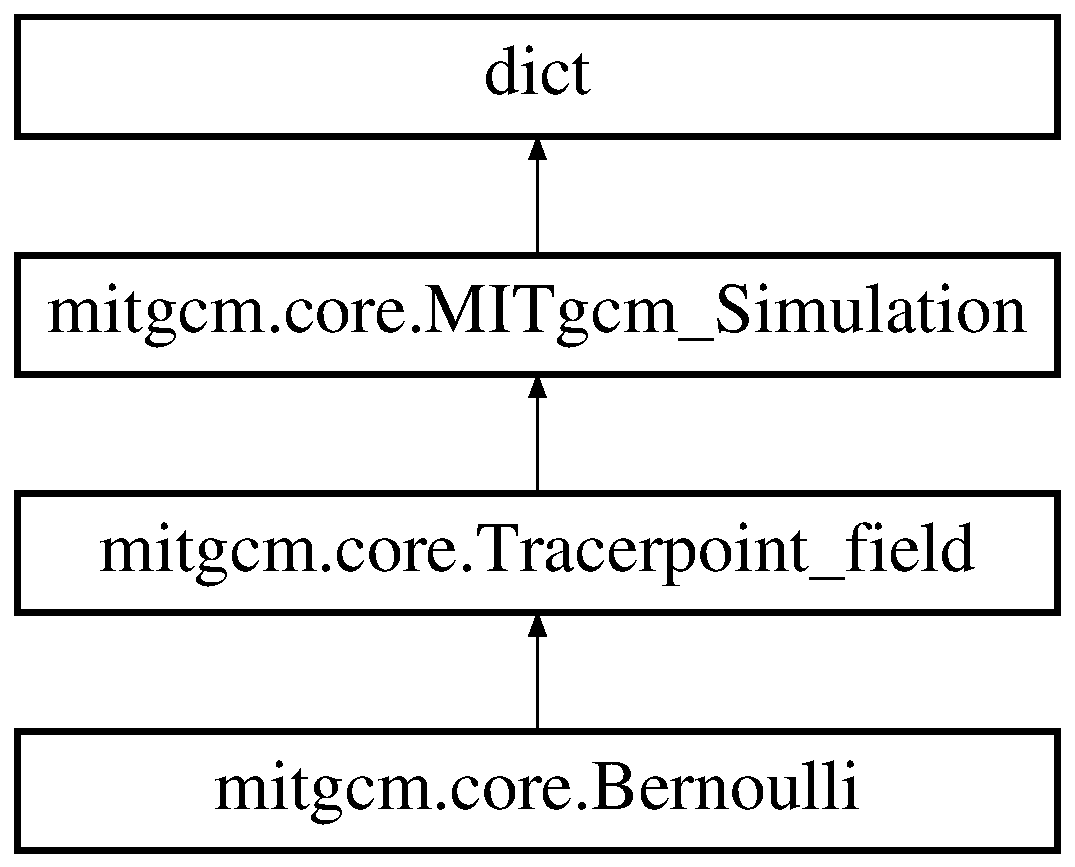
\includegraphics[height=4.000000cm]{classmitgcm_1_1core_1_1Bernoulli}
\end{center}
\end{figure}
\subsection*{Public Member Functions}
\begin{DoxyCompactItemize}
\item 
def \hyperlink{classmitgcm_1_1core_1_1Bernoulli_a823e52977dd3ac349fb569eb3a4bf167}{\+\_\+\+\_\+init\+\_\+\+\_\+}
\end{DoxyCompactItemize}
\subsection*{Additional Inherited Members}


\subsection{Detailed Description}
The \hyperlink{classmitgcm_1_1core_1_1Bernoulli}{Bernoulli} field, evaluated from velocity, pressure and density. 



Definition at line 812 of file core.\+py.



\subsection{Constructor \& Destructor Documentation}
\hypertarget{classmitgcm_1_1core_1_1Bernoulli_a823e52977dd3ac349fb569eb3a4bf167}{}\index{mitgcm\+::core\+::\+Bernoulli@{mitgcm\+::core\+::\+Bernoulli}!\+\_\+\+\_\+init\+\_\+\+\_\+@{\+\_\+\+\_\+init\+\_\+\+\_\+}}
\index{\+\_\+\+\_\+init\+\_\+\+\_\+@{\+\_\+\+\_\+init\+\_\+\+\_\+}!mitgcm\+::core\+::\+Bernoulli@{mitgcm\+::core\+::\+Bernoulli}}
\subsubsection[{\+\_\+\+\_\+init\+\_\+\+\_\+}]{\setlength{\rightskip}{0pt plus 5cm}def mitgcm.\+core.\+Bernoulli.\+\_\+\+\_\+init\+\_\+\+\_\+ (
\begin{DoxyParamCaption}
\item[{}]{self, }
\item[{}]{model\+\_\+instance, }
\item[{}]{density\+\_\+field = {\ttfamily \textquotesingle{}RHO\textquotesingle{}}, }
\item[{}]{U\+V\+E\+L\+\_\+field = {\ttfamily \textquotesingle{}UVEL\textquotesingle{}}, }
\item[{}]{V\+V\+E\+L\+\_\+field = {\ttfamily \textquotesingle{}VVEL\textquotesingle{}}}
\end{DoxyParamCaption}
)}\label{classmitgcm_1_1core_1_1Bernoulli_a823e52977dd3ac349fb569eb3a4bf167}


Definition at line 813 of file core.\+py.



The documentation for this class was generated from the following file\+:\begin{DoxyCompactItemize}
\item 
\hyperlink{core_8py}{core.\+py}\end{DoxyCompactItemize}

\hypertarget{classmitgcm_1_1core_1_1Density}{\section{mitgcm.\+core.\+Density Class Reference}
\label{classmitgcm_1_1core_1_1Density}\index{mitgcm.\+core.\+Density@{mitgcm.\+core.\+Density}}
}
Inheritance diagram for mitgcm.\+core.\+Density\+:\begin{figure}[H]
\begin{center}
\leavevmode
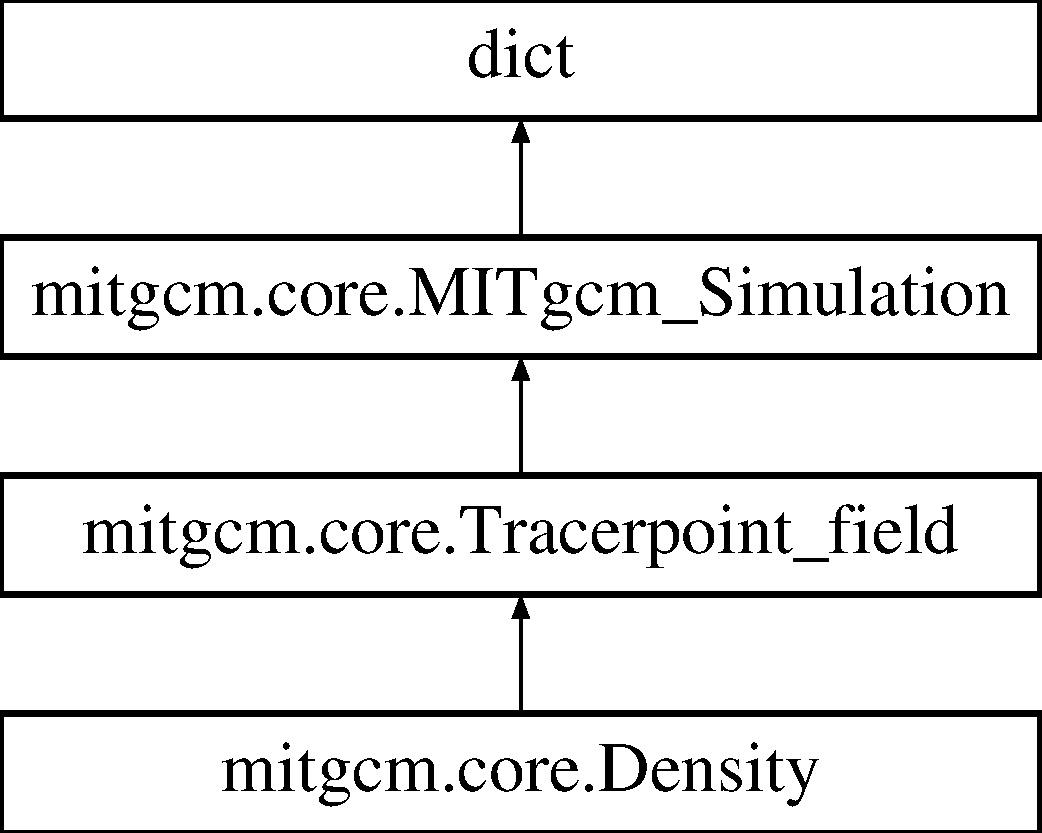
\includegraphics[height=4.000000cm]{classmitgcm_1_1core_1_1Density}
\end{center}
\end{figure}
\subsection*{Public Member Functions}
\begin{DoxyCompactItemize}
\item 
def \hyperlink{classmitgcm_1_1core_1_1Density_ac4f90f6a9c4a9fe9608b5bfdcb09a47c}{\+\_\+\+\_\+init\+\_\+\+\_\+}
\item 
def \hyperlink{classmitgcm_1_1core_1_1Density_aa8d1673db5cfbcd7fda25ad38a29b3a8}{calculate\+\_\+\+Tot\+Rho\+Tend}
\end{DoxyCompactItemize}
\subsection*{Additional Inherited Members}


\subsection{Detailed Description}


Definition at line 642 of file core.\+py.



\subsection{Constructor \& Destructor Documentation}
\hypertarget{classmitgcm_1_1core_1_1Density_ac4f90f6a9c4a9fe9608b5bfdcb09a47c}{\index{mitgcm\+::core\+::\+Density@{mitgcm\+::core\+::\+Density}!\+\_\+\+\_\+init\+\_\+\+\_\+@{\+\_\+\+\_\+init\+\_\+\+\_\+}}
\index{\+\_\+\+\_\+init\+\_\+\+\_\+@{\+\_\+\+\_\+init\+\_\+\+\_\+}!mitgcm\+::core\+::\+Density@{mitgcm\+::core\+::\+Density}}
\subsubsection[{\+\_\+\+\_\+init\+\_\+\+\_\+}]{\setlength{\rightskip}{0pt plus 5cm}def mitgcm.\+core.\+Density.\+\_\+\+\_\+init\+\_\+\+\_\+ (
\begin{DoxyParamCaption}
\item[{}]{self, }
\item[{}]{model\+\_\+instance, }
\item[{}]{Talpha = {\ttfamily 2e-\/4}, }
\item[{}]{Sbeta = {\ttfamily 0}, }
\item[{}]{Rho\+Nil = {\ttfamily 1035}, }
\item[{}]{cp = {\ttfamily 4000}}
\end{DoxyParamCaption}
)}}\label{classmitgcm_1_1core_1_1Density_ac4f90f6a9c4a9fe9608b5bfdcb09a47c}


Definition at line 643 of file core.\+py.



\subsection{Member Function Documentation}
\hypertarget{classmitgcm_1_1core_1_1Density_aa8d1673db5cfbcd7fda25ad38a29b3a8}{\index{mitgcm\+::core\+::\+Density@{mitgcm\+::core\+::\+Density}!calculate\+\_\+\+Tot\+Rho\+Tend@{calculate\+\_\+\+Tot\+Rho\+Tend}}
\index{calculate\+\_\+\+Tot\+Rho\+Tend@{calculate\+\_\+\+Tot\+Rho\+Tend}!mitgcm\+::core\+::\+Density@{mitgcm\+::core\+::\+Density}}
\subsubsection[{calculate\+\_\+\+Tot\+Rho\+Tend}]{\setlength{\rightskip}{0pt plus 5cm}def mitgcm.\+core.\+Density.\+calculate\+\_\+\+Tot\+Rho\+Tend (
\begin{DoxyParamCaption}
\item[{}]{self, }
\item[{}]{model\+\_\+instance}
\end{DoxyParamCaption}
)}}\label{classmitgcm_1_1core_1_1Density_aa8d1673db5cfbcd7fda25ad38a29b3a8}


Definition at line 660 of file core.\+py.



The documentation for this class was generated from the following file\+:\begin{DoxyCompactItemize}
\item 
\hyperlink{core_8py}{core.\+py}\end{DoxyCompactItemize}

\hypertarget{classmitgcm_1_1core_1_1Free__surface}{\section{mitgcm.\+core.\+Free\+\_\+surface Class Reference}
\label{classmitgcm_1_1core_1_1Free__surface}\index{mitgcm.\+core.\+Free\+\_\+surface@{mitgcm.\+core.\+Free\+\_\+surface}}
}
Inheritance diagram for mitgcm.\+core.\+Free\+\_\+surface\+:\begin{figure}[H]
\begin{center}
\leavevmode
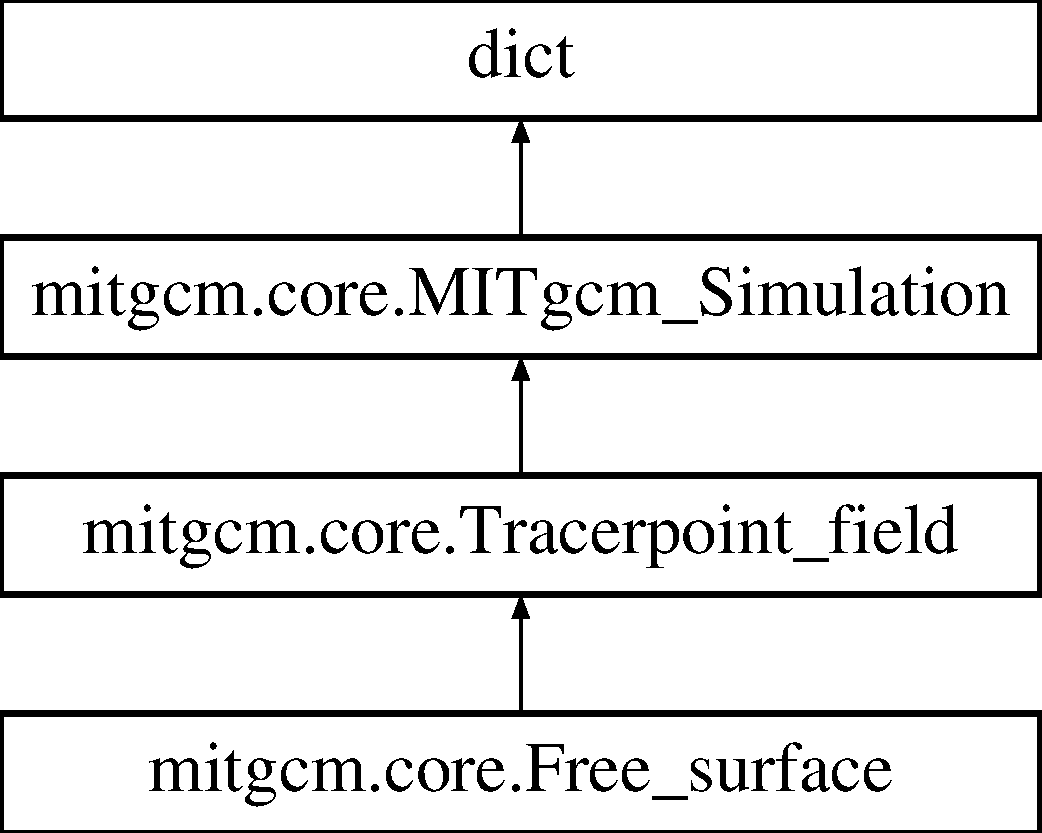
\includegraphics[height=4.000000cm]{classmitgcm_1_1core_1_1Free__surface}
\end{center}
\end{figure}
\subsection*{Public Member Functions}
\begin{DoxyCompactItemize}
\item 
def \hyperlink{classmitgcm_1_1core_1_1Free__surface_aae91ac10ad70025da71f3694f063ec8b}{\+\_\+\+\_\+init\+\_\+\+\_\+}
\end{DoxyCompactItemize}
\subsection*{Additional Inherited Members}


\subsection{Detailed Description}


Definition at line 716 of file core.\+py.



\subsection{Constructor \& Destructor Documentation}
\hypertarget{classmitgcm_1_1core_1_1Free__surface_aae91ac10ad70025da71f3694f063ec8b}{\index{mitgcm\+::core\+::\+Free\+\_\+surface@{mitgcm\+::core\+::\+Free\+\_\+surface}!\+\_\+\+\_\+init\+\_\+\+\_\+@{\+\_\+\+\_\+init\+\_\+\+\_\+}}
\index{\+\_\+\+\_\+init\+\_\+\+\_\+@{\+\_\+\+\_\+init\+\_\+\+\_\+}!mitgcm\+::core\+::\+Free\+\_\+surface@{mitgcm\+::core\+::\+Free\+\_\+surface}}
\subsubsection[{\+\_\+\+\_\+init\+\_\+\+\_\+}]{\setlength{\rightskip}{0pt plus 5cm}def mitgcm.\+core.\+Free\+\_\+surface.\+\_\+\+\_\+init\+\_\+\+\_\+ (
\begin{DoxyParamCaption}
\item[{}]{self, }
\item[{}]{netcdf\+\_\+filename, }
\item[{}]{variable, }
\item[{}]{time\+\_\+level, }
\item[{}]{empty = {\ttfamily False}}
\end{DoxyParamCaption}
)}}\label{classmitgcm_1_1core_1_1Free__surface_aae91ac10ad70025da71f3694f063ec8b}


Definition at line 717 of file core.\+py.



The documentation for this class was generated from the following file\+:\begin{DoxyCompactItemize}
\item 
\hyperlink{core_8py}{core.\+py}\end{DoxyCompactItemize}

\hypertarget{classmitgcm_1_1core_1_1Grid}{\section{mitgcm.\+core.\+Grid Class Reference}
\label{classmitgcm_1_1core_1_1Grid}\index{mitgcm.\+core.\+Grid@{mitgcm.\+core.\+Grid}}
}


This defines the class for the grid object.  


Inheritance diagram for mitgcm.\+core.\+Grid\+:\begin{figure}[H]
\begin{center}
\leavevmode
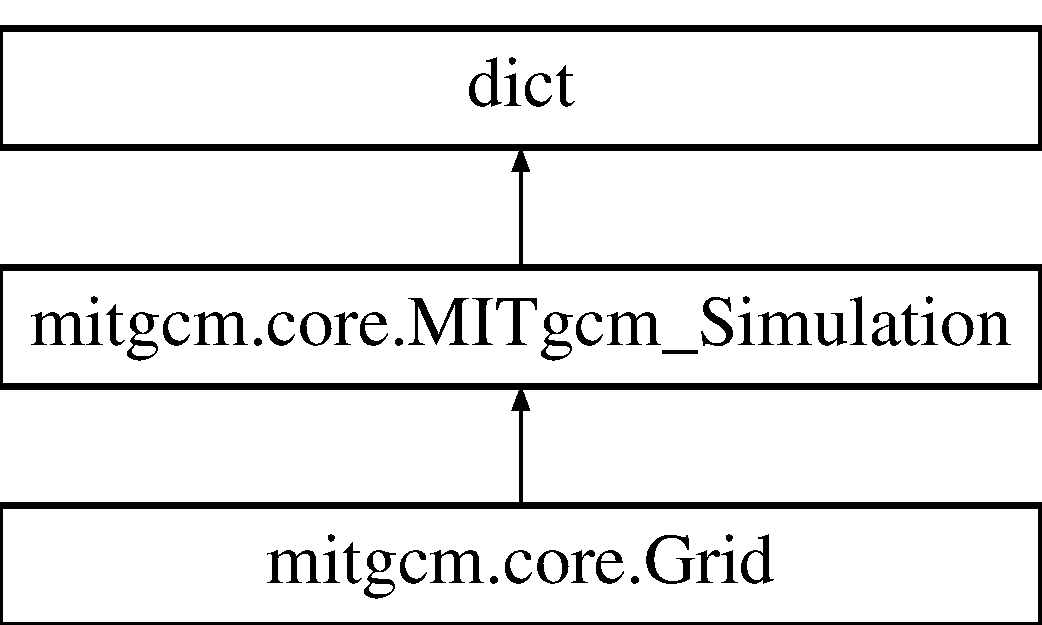
\includegraphics[height=3.000000cm]{classmitgcm_1_1core_1_1Grid}
\end{center}
\end{figure}
\subsection*{Public Member Functions}
\begin{DoxyCompactItemize}
\item 
def \hyperlink{classmitgcm_1_1core_1_1Grid_a8697cc503024a546e189c2707c56c0db}{\+\_\+\+\_\+init\+\_\+\+\_\+}
\begin{DoxyCompactList}\small\item\em Define a single object that has all of the grid variables tucked away in it. \end{DoxyCompactList}\end{DoxyCompactItemize}
\subsection*{Public Attributes}
\begin{DoxyCompactItemize}
\item 
\hyperlink{classmitgcm_1_1core_1_1Grid_adbed7b029a384434aca96fc553ded624}{r\+Aw}
\item 
\hyperlink{classmitgcm_1_1core_1_1Grid_a39b86150afe4e5d57702c86329cf3280}{r\+As}
\item 
\hyperlink{classmitgcm_1_1core_1_1Grid_adc031f161f566cb07d37c5a8a24b7e17}{r\+A}
\item 
\hyperlink{classmitgcm_1_1core_1_1Grid_a8c2c688d2378fe573e6e05db31c17cd2}{H\+Fac\+W}
\item 
\hyperlink{classmitgcm_1_1core_1_1Grid_a684f5d212fd29f4eb3432b491b95a82c}{H\+Fac\+S}
\item 
\hyperlink{classmitgcm_1_1core_1_1Grid_a757d09330b819c4650085004dede249e}{H\+Fac\+C}
\item 
\hyperlink{classmitgcm_1_1core_1_1Grid_a7787160106944191d5a4663774854f49}{X}
\item 
\hyperlink{classmitgcm_1_1core_1_1Grid_ab776eda0111565ec823081cfb9654867}{Xp1}
\item 
\hyperlink{classmitgcm_1_1core_1_1Grid_a39285f6f566718178d156838e1c10ee7}{dx\+F}
\item 
\hyperlink{classmitgcm_1_1core_1_1Grid_a5df9ec1a09a18057a0f2f9459fac9375}{dx\+C}
\item 
\hyperlink{classmitgcm_1_1core_1_1Grid_a6d7d2f28292d3b317519fcf83cb8ade9}{dx\+V}
\item 
\hyperlink{classmitgcm_1_1core_1_1Grid_aee6500dc4e99c849fab046c01a3ba25f}{Y}
\item 
\hyperlink{classmitgcm_1_1core_1_1Grid_a7a2b21d780a2a2152bcb381241778964}{dy\+U}
\item 
\hyperlink{classmitgcm_1_1core_1_1Grid_aaed4fc20f0d9bfee00e1da34032d8a98}{dy\+C}
\item 
\hyperlink{classmitgcm_1_1core_1_1Grid_ac6198e01c8d9e3c491afa9c7d2162a45}{dy\+F}
\item 
\hyperlink{classmitgcm_1_1core_1_1Grid_a7486bee7b120f39baa0bc84e663291fe}{Z}
\item 
\hyperlink{classmitgcm_1_1core_1_1Grid_aea2f7ddb0b140ad791b7ce7f96569bd9}{Zl}
\item 
\hyperlink{classmitgcm_1_1core_1_1Grid_a997f5082eb939242633601aa45a28744}{Zu}
\item 
\hyperlink{classmitgcm_1_1core_1_1Grid_aecdb2f77448391f837648248342fbc28}{dr\+C}
\item 
\hyperlink{classmitgcm_1_1core_1_1Grid_a75699b4c667aaa6e04c6a0504c6b62ea}{dr\+F}
\item 
\hyperlink{classmitgcm_1_1core_1_1Grid_ad62c4a7ffebe74f9c017b238d3d6ec16}{f\+Cori\+G}
\item 
\hyperlink{classmitgcm_1_1core_1_1Grid_a924a827552b8bfcc08c750637364224f}{wet\+\_\+mask\+\_\+\+V}
\item 
\hyperlink{classmitgcm_1_1core_1_1Grid_aaa07d628d03ff550e2a711ed62dcfc55}{wet\+\_\+mask\+\_\+\+U}
\item 
\hyperlink{classmitgcm_1_1core_1_1Grid_a4f7637908d982efab96f34c32fed20bd}{wet\+\_\+mask\+\_\+\+T\+H}
\item 
\hyperlink{classmitgcm_1_1core_1_1Grid_ada3063facd1f0f929237bf1589224121}{wet\+\_\+mask\+\_\+\+W}
\item 
\hyperlink{classmitgcm_1_1core_1_1Grid_a09a2f1e06b6d74ebd1779140351136a9}{cell\+\_\+volume}
\item 
\hyperlink{classmitgcm_1_1core_1_1Grid_ac9afe3373e16ca1b8343f8669b9eb4bb}{west\+\_\+mask}
\item 
\hyperlink{classmitgcm_1_1core_1_1Grid_ab2303190a4150bf2c67450e6f5514624}{east\+\_\+mask}
\item 
\hyperlink{classmitgcm_1_1core_1_1Grid_a4f70506e6225a48f53c4f57299ad0da8}{south\+\_\+mask}
\item 
\hyperlink{classmitgcm_1_1core_1_1Grid_ade43e2fe2061d12e5945dffee14d7378}{north\+\_\+mask}
\item 
\hyperlink{classmitgcm_1_1core_1_1Grid_a69f90f4bcf5c06fab90674814eff4de9}{bottom\+\_\+mask}
\end{DoxyCompactItemize}


\subsection{Detailed Description}
This defines the class for the grid object. 

This object holds all the information about the grid on which the simulation was run. It also holds mask for getting only the boundary values of fields on the tracer points. \begin{DoxyVerb}This class is the only one that isn't written to use dicts - this should be fixed at some stage. \end{DoxyVerb}
 

Definition at line 547 of file core.\+py.



\subsection{Constructor \& Destructor Documentation}
\hypertarget{classmitgcm_1_1core_1_1Grid_a8697cc503024a546e189c2707c56c0db}{\index{mitgcm\+::core\+::\+Grid@{mitgcm\+::core\+::\+Grid}!\+\_\+\+\_\+init\+\_\+\+\_\+@{\+\_\+\+\_\+init\+\_\+\+\_\+}}
\index{\+\_\+\+\_\+init\+\_\+\+\_\+@{\+\_\+\+\_\+init\+\_\+\+\_\+}!mitgcm\+::core\+::\+Grid@{mitgcm\+::core\+::\+Grid}}
\subsubsection[{\+\_\+\+\_\+init\+\_\+\+\_\+}]{\setlength{\rightskip}{0pt plus 5cm}def mitgcm.\+core.\+Grid.\+\_\+\+\_\+init\+\_\+\+\_\+ (
\begin{DoxyParamCaption}
\item[{}]{self, }
\item[{}]{grid\+\_\+netcdf\+\_\+filename}
\end{DoxyParamCaption}
)}}\label{classmitgcm_1_1core_1_1Grid_a8697cc503024a546e189c2707c56c0db}


Define a single object that has all of the grid variables tucked away in it. 

Each of the variables pulled directly from the netcdf file still has the original description attached to it. The 2\+D and 3\+D arrays do not. 

Definition at line 553 of file core.\+py.



\subsection{Member Data Documentation}
\hypertarget{classmitgcm_1_1core_1_1Grid_a69f90f4bcf5c06fab90674814eff4de9}{\index{mitgcm\+::core\+::\+Grid@{mitgcm\+::core\+::\+Grid}!bottom\+\_\+mask@{bottom\+\_\+mask}}
\index{bottom\+\_\+mask@{bottom\+\_\+mask}!mitgcm\+::core\+::\+Grid@{mitgcm\+::core\+::\+Grid}}
\subsubsection[{bottom\+\_\+mask}]{\setlength{\rightskip}{0pt plus 5cm}mitgcm.\+core.\+Grid.\+bottom\+\_\+mask}}\label{classmitgcm_1_1core_1_1Grid_a69f90f4bcf5c06fab90674814eff4de9}


Definition at line 598 of file core.\+py.

\hypertarget{classmitgcm_1_1core_1_1Grid_a09a2f1e06b6d74ebd1779140351136a9}{\index{mitgcm\+::core\+::\+Grid@{mitgcm\+::core\+::\+Grid}!cell\+\_\+volume@{cell\+\_\+volume}}
\index{cell\+\_\+volume@{cell\+\_\+volume}!mitgcm\+::core\+::\+Grid@{mitgcm\+::core\+::\+Grid}}
\subsubsection[{cell\+\_\+volume}]{\setlength{\rightskip}{0pt plus 5cm}mitgcm.\+core.\+Grid.\+cell\+\_\+volume}}\label{classmitgcm_1_1core_1_1Grid_a09a2f1e06b6d74ebd1779140351136a9}


Definition at line 592 of file core.\+py.

\hypertarget{classmitgcm_1_1core_1_1Grid_aecdb2f77448391f837648248342fbc28}{\index{mitgcm\+::core\+::\+Grid@{mitgcm\+::core\+::\+Grid}!dr\+C@{dr\+C}}
\index{dr\+C@{dr\+C}!mitgcm\+::core\+::\+Grid@{mitgcm\+::core\+::\+Grid}}
\subsubsection[{dr\+C}]{\setlength{\rightskip}{0pt plus 5cm}mitgcm.\+core.\+Grid.\+dr\+C}}\label{classmitgcm_1_1core_1_1Grid_aecdb2f77448391f837648248342fbc28}


Definition at line 573 of file core.\+py.

\hypertarget{classmitgcm_1_1core_1_1Grid_a75699b4c667aaa6e04c6a0504c6b62ea}{\index{mitgcm\+::core\+::\+Grid@{mitgcm\+::core\+::\+Grid}!dr\+F@{dr\+F}}
\index{dr\+F@{dr\+F}!mitgcm\+::core\+::\+Grid@{mitgcm\+::core\+::\+Grid}}
\subsubsection[{dr\+F}]{\setlength{\rightskip}{0pt plus 5cm}mitgcm.\+core.\+Grid.\+dr\+F}}\label{classmitgcm_1_1core_1_1Grid_a75699b4c667aaa6e04c6a0504c6b62ea}


Definition at line 574 of file core.\+py.

\hypertarget{classmitgcm_1_1core_1_1Grid_a5df9ec1a09a18057a0f2f9459fac9375}{\index{mitgcm\+::core\+::\+Grid@{mitgcm\+::core\+::\+Grid}!dx\+C@{dx\+C}}
\index{dx\+C@{dx\+C}!mitgcm\+::core\+::\+Grid@{mitgcm\+::core\+::\+Grid}}
\subsubsection[{dx\+C}]{\setlength{\rightskip}{0pt plus 5cm}mitgcm.\+core.\+Grid.\+dx\+C}}\label{classmitgcm_1_1core_1_1Grid_a5df9ec1a09a18057a0f2f9459fac9375}


Definition at line 564 of file core.\+py.

\hypertarget{classmitgcm_1_1core_1_1Grid_a39285f6f566718178d156838e1c10ee7}{\index{mitgcm\+::core\+::\+Grid@{mitgcm\+::core\+::\+Grid}!dx\+F@{dx\+F}}
\index{dx\+F@{dx\+F}!mitgcm\+::core\+::\+Grid@{mitgcm\+::core\+::\+Grid}}
\subsubsection[{dx\+F}]{\setlength{\rightskip}{0pt plus 5cm}mitgcm.\+core.\+Grid.\+dx\+F}}\label{classmitgcm_1_1core_1_1Grid_a39285f6f566718178d156838e1c10ee7}


Definition at line 563 of file core.\+py.

\hypertarget{classmitgcm_1_1core_1_1Grid_a6d7d2f28292d3b317519fcf83cb8ade9}{\index{mitgcm\+::core\+::\+Grid@{mitgcm\+::core\+::\+Grid}!dx\+V@{dx\+V}}
\index{dx\+V@{dx\+V}!mitgcm\+::core\+::\+Grid@{mitgcm\+::core\+::\+Grid}}
\subsubsection[{dx\+V}]{\setlength{\rightskip}{0pt plus 5cm}mitgcm.\+core.\+Grid.\+dx\+V}}\label{classmitgcm_1_1core_1_1Grid_a6d7d2f28292d3b317519fcf83cb8ade9}


Definition at line 565 of file core.\+py.

\hypertarget{classmitgcm_1_1core_1_1Grid_aaed4fc20f0d9bfee00e1da34032d8a98}{\index{mitgcm\+::core\+::\+Grid@{mitgcm\+::core\+::\+Grid}!dy\+C@{dy\+C}}
\index{dy\+C@{dy\+C}!mitgcm\+::core\+::\+Grid@{mitgcm\+::core\+::\+Grid}}
\subsubsection[{dy\+C}]{\setlength{\rightskip}{0pt plus 5cm}mitgcm.\+core.\+Grid.\+dy\+C}}\label{classmitgcm_1_1core_1_1Grid_aaed4fc20f0d9bfee00e1da34032d8a98}


Definition at line 568 of file core.\+py.

\hypertarget{classmitgcm_1_1core_1_1Grid_ac6198e01c8d9e3c491afa9c7d2162a45}{\index{mitgcm\+::core\+::\+Grid@{mitgcm\+::core\+::\+Grid}!dy\+F@{dy\+F}}
\index{dy\+F@{dy\+F}!mitgcm\+::core\+::\+Grid@{mitgcm\+::core\+::\+Grid}}
\subsubsection[{dy\+F}]{\setlength{\rightskip}{0pt plus 5cm}mitgcm.\+core.\+Grid.\+dy\+F}}\label{classmitgcm_1_1core_1_1Grid_ac6198e01c8d9e3c491afa9c7d2162a45}


Definition at line 569 of file core.\+py.

\hypertarget{classmitgcm_1_1core_1_1Grid_a7a2b21d780a2a2152bcb381241778964}{\index{mitgcm\+::core\+::\+Grid@{mitgcm\+::core\+::\+Grid}!dy\+U@{dy\+U}}
\index{dy\+U@{dy\+U}!mitgcm\+::core\+::\+Grid@{mitgcm\+::core\+::\+Grid}}
\subsubsection[{dy\+U}]{\setlength{\rightskip}{0pt plus 5cm}mitgcm.\+core.\+Grid.\+dy\+U}}\label{classmitgcm_1_1core_1_1Grid_a7a2b21d780a2a2152bcb381241778964}


Definition at line 567 of file core.\+py.

\hypertarget{classmitgcm_1_1core_1_1Grid_ab2303190a4150bf2c67450e6f5514624}{\index{mitgcm\+::core\+::\+Grid@{mitgcm\+::core\+::\+Grid}!east\+\_\+mask@{east\+\_\+mask}}
\index{east\+\_\+mask@{east\+\_\+mask}!mitgcm\+::core\+::\+Grid@{mitgcm\+::core\+::\+Grid}}
\subsubsection[{east\+\_\+mask}]{\setlength{\rightskip}{0pt plus 5cm}mitgcm.\+core.\+Grid.\+east\+\_\+mask}}\label{classmitgcm_1_1core_1_1Grid_ab2303190a4150bf2c67450e6f5514624}


Definition at line 595 of file core.\+py.

\hypertarget{classmitgcm_1_1core_1_1Grid_ad62c4a7ffebe74f9c017b238d3d6ec16}{\index{mitgcm\+::core\+::\+Grid@{mitgcm\+::core\+::\+Grid}!f\+Cori\+G@{f\+Cori\+G}}
\index{f\+Cori\+G@{f\+Cori\+G}!mitgcm\+::core\+::\+Grid@{mitgcm\+::core\+::\+Grid}}
\subsubsection[{f\+Cori\+G}]{\setlength{\rightskip}{0pt plus 5cm}mitgcm.\+core.\+Grid.\+f\+Cori\+G}}\label{classmitgcm_1_1core_1_1Grid_ad62c4a7ffebe74f9c017b238d3d6ec16}


Definition at line 575 of file core.\+py.

\hypertarget{classmitgcm_1_1core_1_1Grid_a757d09330b819c4650085004dede249e}{\index{mitgcm\+::core\+::\+Grid@{mitgcm\+::core\+::\+Grid}!H\+Fac\+C@{H\+Fac\+C}}
\index{H\+Fac\+C@{H\+Fac\+C}!mitgcm\+::core\+::\+Grid@{mitgcm\+::core\+::\+Grid}}
\subsubsection[{H\+Fac\+C}]{\setlength{\rightskip}{0pt plus 5cm}mitgcm.\+core.\+Grid.\+H\+Fac\+C}}\label{classmitgcm_1_1core_1_1Grid_a757d09330b819c4650085004dede249e}


Definition at line 560 of file core.\+py.

\hypertarget{classmitgcm_1_1core_1_1Grid_a684f5d212fd29f4eb3432b491b95a82c}{\index{mitgcm\+::core\+::\+Grid@{mitgcm\+::core\+::\+Grid}!H\+Fac\+S@{H\+Fac\+S}}
\index{H\+Fac\+S@{H\+Fac\+S}!mitgcm\+::core\+::\+Grid@{mitgcm\+::core\+::\+Grid}}
\subsubsection[{H\+Fac\+S}]{\setlength{\rightskip}{0pt plus 5cm}mitgcm.\+core.\+Grid.\+H\+Fac\+S}}\label{classmitgcm_1_1core_1_1Grid_a684f5d212fd29f4eb3432b491b95a82c}


Definition at line 559 of file core.\+py.

\hypertarget{classmitgcm_1_1core_1_1Grid_a8c2c688d2378fe573e6e05db31c17cd2}{\index{mitgcm\+::core\+::\+Grid@{mitgcm\+::core\+::\+Grid}!H\+Fac\+W@{H\+Fac\+W}}
\index{H\+Fac\+W@{H\+Fac\+W}!mitgcm\+::core\+::\+Grid@{mitgcm\+::core\+::\+Grid}}
\subsubsection[{H\+Fac\+W}]{\setlength{\rightskip}{0pt plus 5cm}mitgcm.\+core.\+Grid.\+H\+Fac\+W}}\label{classmitgcm_1_1core_1_1Grid_a8c2c688d2378fe573e6e05db31c17cd2}


Definition at line 558 of file core.\+py.

\hypertarget{classmitgcm_1_1core_1_1Grid_ade43e2fe2061d12e5945dffee14d7378}{\index{mitgcm\+::core\+::\+Grid@{mitgcm\+::core\+::\+Grid}!north\+\_\+mask@{north\+\_\+mask}}
\index{north\+\_\+mask@{north\+\_\+mask}!mitgcm\+::core\+::\+Grid@{mitgcm\+::core\+::\+Grid}}
\subsubsection[{north\+\_\+mask}]{\setlength{\rightskip}{0pt plus 5cm}mitgcm.\+core.\+Grid.\+north\+\_\+mask}}\label{classmitgcm_1_1core_1_1Grid_ade43e2fe2061d12e5945dffee14d7378}


Definition at line 597 of file core.\+py.

\hypertarget{classmitgcm_1_1core_1_1Grid_adc031f161f566cb07d37c5a8a24b7e17}{\index{mitgcm\+::core\+::\+Grid@{mitgcm\+::core\+::\+Grid}!r\+A@{r\+A}}
\index{r\+A@{r\+A}!mitgcm\+::core\+::\+Grid@{mitgcm\+::core\+::\+Grid}}
\subsubsection[{r\+A}]{\setlength{\rightskip}{0pt plus 5cm}mitgcm.\+core.\+Grid.\+r\+A}}\label{classmitgcm_1_1core_1_1Grid_adc031f161f566cb07d37c5a8a24b7e17}


Definition at line 557 of file core.\+py.

\hypertarget{classmitgcm_1_1core_1_1Grid_a39b86150afe4e5d57702c86329cf3280}{\index{mitgcm\+::core\+::\+Grid@{mitgcm\+::core\+::\+Grid}!r\+As@{r\+As}}
\index{r\+As@{r\+As}!mitgcm\+::core\+::\+Grid@{mitgcm\+::core\+::\+Grid}}
\subsubsection[{r\+As}]{\setlength{\rightskip}{0pt plus 5cm}mitgcm.\+core.\+Grid.\+r\+As}}\label{classmitgcm_1_1core_1_1Grid_a39b86150afe4e5d57702c86329cf3280}


Definition at line 556 of file core.\+py.

\hypertarget{classmitgcm_1_1core_1_1Grid_adbed7b029a384434aca96fc553ded624}{\index{mitgcm\+::core\+::\+Grid@{mitgcm\+::core\+::\+Grid}!r\+Aw@{r\+Aw}}
\index{r\+Aw@{r\+Aw}!mitgcm\+::core\+::\+Grid@{mitgcm\+::core\+::\+Grid}}
\subsubsection[{r\+Aw}]{\setlength{\rightskip}{0pt plus 5cm}mitgcm.\+core.\+Grid.\+r\+Aw}}\label{classmitgcm_1_1core_1_1Grid_adbed7b029a384434aca96fc553ded624}


Definition at line 555 of file core.\+py.

\hypertarget{classmitgcm_1_1core_1_1Grid_a4f70506e6225a48f53c4f57299ad0da8}{\index{mitgcm\+::core\+::\+Grid@{mitgcm\+::core\+::\+Grid}!south\+\_\+mask@{south\+\_\+mask}}
\index{south\+\_\+mask@{south\+\_\+mask}!mitgcm\+::core\+::\+Grid@{mitgcm\+::core\+::\+Grid}}
\subsubsection[{south\+\_\+mask}]{\setlength{\rightskip}{0pt plus 5cm}mitgcm.\+core.\+Grid.\+south\+\_\+mask}}\label{classmitgcm_1_1core_1_1Grid_a4f70506e6225a48f53c4f57299ad0da8}


Definition at line 596 of file core.\+py.

\hypertarget{classmitgcm_1_1core_1_1Grid_ac9afe3373e16ca1b8343f8669b9eb4bb}{\index{mitgcm\+::core\+::\+Grid@{mitgcm\+::core\+::\+Grid}!west\+\_\+mask@{west\+\_\+mask}}
\index{west\+\_\+mask@{west\+\_\+mask}!mitgcm\+::core\+::\+Grid@{mitgcm\+::core\+::\+Grid}}
\subsubsection[{west\+\_\+mask}]{\setlength{\rightskip}{0pt plus 5cm}mitgcm.\+core.\+Grid.\+west\+\_\+mask}}\label{classmitgcm_1_1core_1_1Grid_ac9afe3373e16ca1b8343f8669b9eb4bb}


Definition at line 594 of file core.\+py.

\hypertarget{classmitgcm_1_1core_1_1Grid_a4f7637908d982efab96f34c32fed20bd}{\index{mitgcm\+::core\+::\+Grid@{mitgcm\+::core\+::\+Grid}!wet\+\_\+mask\+\_\+\+T\+H@{wet\+\_\+mask\+\_\+\+T\+H}}
\index{wet\+\_\+mask\+\_\+\+T\+H@{wet\+\_\+mask\+\_\+\+T\+H}!mitgcm\+::core\+::\+Grid@{mitgcm\+::core\+::\+Grid}}
\subsubsection[{wet\+\_\+mask\+\_\+\+T\+H}]{\setlength{\rightskip}{0pt plus 5cm}mitgcm.\+core.\+Grid.\+wet\+\_\+mask\+\_\+\+T\+H}}\label{classmitgcm_1_1core_1_1Grid_a4f7637908d982efab96f34c32fed20bd}


Definition at line 588 of file core.\+py.

\hypertarget{classmitgcm_1_1core_1_1Grid_aaa07d628d03ff550e2a711ed62dcfc55}{\index{mitgcm\+::core\+::\+Grid@{mitgcm\+::core\+::\+Grid}!wet\+\_\+mask\+\_\+\+U@{wet\+\_\+mask\+\_\+\+U}}
\index{wet\+\_\+mask\+\_\+\+U@{wet\+\_\+mask\+\_\+\+U}!mitgcm\+::core\+::\+Grid@{mitgcm\+::core\+::\+Grid}}
\subsubsection[{wet\+\_\+mask\+\_\+\+U}]{\setlength{\rightskip}{0pt plus 5cm}mitgcm.\+core.\+Grid.\+wet\+\_\+mask\+\_\+\+U}}\label{classmitgcm_1_1core_1_1Grid_aaa07d628d03ff550e2a711ed62dcfc55}


Definition at line 586 of file core.\+py.

\hypertarget{classmitgcm_1_1core_1_1Grid_a924a827552b8bfcc08c750637364224f}{\index{mitgcm\+::core\+::\+Grid@{mitgcm\+::core\+::\+Grid}!wet\+\_\+mask\+\_\+\+V@{wet\+\_\+mask\+\_\+\+V}}
\index{wet\+\_\+mask\+\_\+\+V@{wet\+\_\+mask\+\_\+\+V}!mitgcm\+::core\+::\+Grid@{mitgcm\+::core\+::\+Grid}}
\subsubsection[{wet\+\_\+mask\+\_\+\+V}]{\setlength{\rightskip}{0pt plus 5cm}mitgcm.\+core.\+Grid.\+wet\+\_\+mask\+\_\+\+V}}\label{classmitgcm_1_1core_1_1Grid_a924a827552b8bfcc08c750637364224f}


Definition at line 584 of file core.\+py.

\hypertarget{classmitgcm_1_1core_1_1Grid_ada3063facd1f0f929237bf1589224121}{\index{mitgcm\+::core\+::\+Grid@{mitgcm\+::core\+::\+Grid}!wet\+\_\+mask\+\_\+\+W@{wet\+\_\+mask\+\_\+\+W}}
\index{wet\+\_\+mask\+\_\+\+W@{wet\+\_\+mask\+\_\+\+W}!mitgcm\+::core\+::\+Grid@{mitgcm\+::core\+::\+Grid}}
\subsubsection[{wet\+\_\+mask\+\_\+\+W}]{\setlength{\rightskip}{0pt plus 5cm}mitgcm.\+core.\+Grid.\+wet\+\_\+mask\+\_\+\+W}}\label{classmitgcm_1_1core_1_1Grid_ada3063facd1f0f929237bf1589224121}


Definition at line 590 of file core.\+py.

\hypertarget{classmitgcm_1_1core_1_1Grid_a7787160106944191d5a4663774854f49}{\index{mitgcm\+::core\+::\+Grid@{mitgcm\+::core\+::\+Grid}!X@{X}}
\index{X@{X}!mitgcm\+::core\+::\+Grid@{mitgcm\+::core\+::\+Grid}}
\subsubsection[{X}]{\setlength{\rightskip}{0pt plus 5cm}mitgcm.\+core.\+Grid.\+X}}\label{classmitgcm_1_1core_1_1Grid_a7787160106944191d5a4663774854f49}


Definition at line 561 of file core.\+py.

\hypertarget{classmitgcm_1_1core_1_1Grid_ab776eda0111565ec823081cfb9654867}{\index{mitgcm\+::core\+::\+Grid@{mitgcm\+::core\+::\+Grid}!Xp1@{Xp1}}
\index{Xp1@{Xp1}!mitgcm\+::core\+::\+Grid@{mitgcm\+::core\+::\+Grid}}
\subsubsection[{Xp1}]{\setlength{\rightskip}{0pt plus 5cm}mitgcm.\+core.\+Grid.\+Xp1}}\label{classmitgcm_1_1core_1_1Grid_ab776eda0111565ec823081cfb9654867}


Definition at line 562 of file core.\+py.

\hypertarget{classmitgcm_1_1core_1_1Grid_aee6500dc4e99c849fab046c01a3ba25f}{\index{mitgcm\+::core\+::\+Grid@{mitgcm\+::core\+::\+Grid}!Y@{Y}}
\index{Y@{Y}!mitgcm\+::core\+::\+Grid@{mitgcm\+::core\+::\+Grid}}
\subsubsection[{Y}]{\setlength{\rightskip}{0pt plus 5cm}mitgcm.\+core.\+Grid.\+Y}}\label{classmitgcm_1_1core_1_1Grid_aee6500dc4e99c849fab046c01a3ba25f}


Definition at line 566 of file core.\+py.

\hypertarget{classmitgcm_1_1core_1_1Grid_a7486bee7b120f39baa0bc84e663291fe}{\index{mitgcm\+::core\+::\+Grid@{mitgcm\+::core\+::\+Grid}!Z@{Z}}
\index{Z@{Z}!mitgcm\+::core\+::\+Grid@{mitgcm\+::core\+::\+Grid}}
\subsubsection[{Z}]{\setlength{\rightskip}{0pt plus 5cm}mitgcm.\+core.\+Grid.\+Z}}\label{classmitgcm_1_1core_1_1Grid_a7486bee7b120f39baa0bc84e663291fe}


Definition at line 570 of file core.\+py.

\hypertarget{classmitgcm_1_1core_1_1Grid_aea2f7ddb0b140ad791b7ce7f96569bd9}{\index{mitgcm\+::core\+::\+Grid@{mitgcm\+::core\+::\+Grid}!Zl@{Zl}}
\index{Zl@{Zl}!mitgcm\+::core\+::\+Grid@{mitgcm\+::core\+::\+Grid}}
\subsubsection[{Zl}]{\setlength{\rightskip}{0pt plus 5cm}mitgcm.\+core.\+Grid.\+Zl}}\label{classmitgcm_1_1core_1_1Grid_aea2f7ddb0b140ad791b7ce7f96569bd9}


Definition at line 571 of file core.\+py.

\hypertarget{classmitgcm_1_1core_1_1Grid_a997f5082eb939242633601aa45a28744}{\index{mitgcm\+::core\+::\+Grid@{mitgcm\+::core\+::\+Grid}!Zu@{Zu}}
\index{Zu@{Zu}!mitgcm\+::core\+::\+Grid@{mitgcm\+::core\+::\+Grid}}
\subsubsection[{Zu}]{\setlength{\rightskip}{0pt plus 5cm}mitgcm.\+core.\+Grid.\+Zu}}\label{classmitgcm_1_1core_1_1Grid_a997f5082eb939242633601aa45a28744}


Definition at line 572 of file core.\+py.



The documentation for this class was generated from the following file\+:\begin{DoxyCompactItemize}
\item 
\hyperlink{core_8py}{core.\+py}\end{DoxyCompactItemize}

\hypertarget{classmitgcm_1_1core_1_1MITgcm__Simulation}{\section{mitgcm.\+core.\+M\+I\+Tgcm\+\_\+\+Simulation Class Reference}
\label{classmitgcm_1_1core_1_1MITgcm__Simulation}\index{mitgcm.\+core.\+M\+I\+Tgcm\+\_\+\+Simulation@{mitgcm.\+core.\+M\+I\+Tgcm\+\_\+\+Simulation}}
}


The simulation class is the main class of this package, and an instance of this class is a model object.  


Inheritance diagram for mitgcm.\+core.\+M\+I\+Tgcm\+\_\+\+Simulation\+:\begin{figure}[H]
\begin{center}
\leavevmode
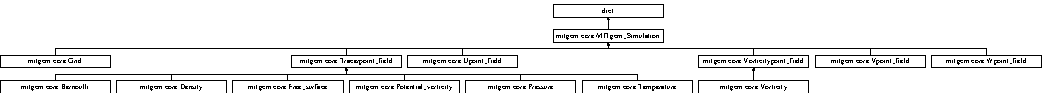
\includegraphics[height=1.244444cm]{classmitgcm_1_1core_1_1MITgcm__Simulation}
\end{center}
\end{figure}
\subsection*{Public Member Functions}
\begin{DoxyCompactItemize}
\item 
def \hyperlink{classmitgcm_1_1core_1_1MITgcm__Simulation_aac012c75a0f5dce8bbc4b00422a12444}{\+\_\+\+\_\+init\+\_\+\+\_\+}
\begin{DoxyCompactList}\small\item\em Instantiate an M\+I\+Tgcm model instance. \end{DoxyCompactList}\item 
def \hyperlink{classmitgcm_1_1core_1_1MITgcm__Simulation_a975760ba1406c74ad06af11ca3925397}{load\+\_\+field}
\begin{DoxyCompactList}\small\item\em Load a model field from Net\+C\+D\+F output. \end{DoxyCompactList}\item 
def \hyperlink{classmitgcm_1_1core_1_1MITgcm__Simulation_a43a67ae2588987ada32f505473d469c8}{\+\_\+\+\_\+add\+\_\+\+\_\+}
\begin{DoxyCompactList}\small\item\em A method that allows model objects to be added together. \end{DoxyCompactList}\item 
def \hyperlink{classmitgcm_1_1core_1_1MITgcm__Simulation_a64a9a65d7ed0ae3344e09dc6a36d41e0}{\+\_\+\+\_\+div\+\_\+\+\_\+}
\begin{DoxyCompactList}\small\item\em A method that allows model objects to be divided by floating point numbers. \end{DoxyCompactList}\item 
def \hyperlink{classmitgcm_1_1core_1_1MITgcm__Simulation_a7827aeb019dd9f93317770e830db03d3}{\+\_\+\+\_\+mul\+\_\+\+\_\+}
\begin{DoxyCompactList}\small\item\em A method that allows model objects to be multiplied by floating point numbers. \end{DoxyCompactList}\item 
def \hyperlink{classmitgcm_1_1core_1_1MITgcm__Simulation_aafdbbd993c0424568a4534edf643d312}{\+\_\+\+\_\+rmul\+\_\+\+\_\+}
\begin{DoxyCompactList}\small\item\em A method that allows model objects to be multiplied by floating point numbers. \end{DoxyCompactList}\end{DoxyCompactItemize}
\subsection*{Public Attributes}
\begin{DoxyCompactItemize}
\item 
\hyperlink{classmitgcm_1_1core_1_1MITgcm__Simulation_a984db65a189bf843e988079f724cdee3}{grid}
\end{DoxyCompactItemize}
\subsection*{Static Public Attributes}
\begin{DoxyCompactItemize}
\item 
tuple \hyperlink{classmitgcm_1_1core_1_1MITgcm__Simulation_a801f2b7847cdd50c031f6f566e263189}{netcdf\+\_\+file} = net\+C\+D\+F4.\+Dataset(netcdf\+\_\+filename)
\item 
list \hyperlink{classmitgcm_1_1core_1_1MITgcm__Simulation_ad50484938272dfc5107b0af495443d25}{loaded\+\_\+field} = netcdf\+\_\+file.\+variables\mbox{[}variable\mbox{]}
\end{DoxyCompactItemize}


\subsection{Detailed Description}
The simulation class is the main class of this package, and an instance of this class is a model object. 

All fields are associated with the model object -\/ either directly (it is a dict), or indirectly through one of its subobjects (which are also dicts). 

Definition at line 29 of file core.\+py.



\subsection{Constructor \& Destructor Documentation}
\hypertarget{classmitgcm_1_1core_1_1MITgcm__Simulation_aac012c75a0f5dce8bbc4b00422a12444}{\index{mitgcm\+::core\+::\+M\+I\+Tgcm\+\_\+\+Simulation@{mitgcm\+::core\+::\+M\+I\+Tgcm\+\_\+\+Simulation}!\+\_\+\+\_\+init\+\_\+\+\_\+@{\+\_\+\+\_\+init\+\_\+\+\_\+}}
\index{\+\_\+\+\_\+init\+\_\+\+\_\+@{\+\_\+\+\_\+init\+\_\+\+\_\+}!mitgcm\+::core\+::\+M\+I\+Tgcm\+\_\+\+Simulation@{mitgcm\+::core\+::\+M\+I\+Tgcm\+\_\+\+Simulation}}
\subsubsection[{\+\_\+\+\_\+init\+\_\+\+\_\+}]{\setlength{\rightskip}{0pt plus 5cm}def mitgcm.\+core.\+M\+I\+Tgcm\+\_\+\+Simulation.\+\_\+\+\_\+init\+\_\+\+\_\+ (
\begin{DoxyParamCaption}
\item[{}]{self, }
\item[{}]{output\+\_\+dir, }
\item[{}]{grid\+\_\+netcdf\+\_\+filename, }
\item[{}]{E\+O\+S\+\_\+type = {\ttfamily 'linear'}, }
\item[{}]{g = {\ttfamily 9.8}}
\end{DoxyParamCaption}
)}}\label{classmitgcm_1_1core_1_1MITgcm__Simulation_aac012c75a0f5dce8bbc4b00422a12444}


Instantiate an M\+I\+Tgcm model instance. 



Definition at line 32 of file core.\+py.



\subsection{Member Function Documentation}
\hypertarget{classmitgcm_1_1core_1_1MITgcm__Simulation_a43a67ae2588987ada32f505473d469c8}{\index{mitgcm\+::core\+::\+M\+I\+Tgcm\+\_\+\+Simulation@{mitgcm\+::core\+::\+M\+I\+Tgcm\+\_\+\+Simulation}!\+\_\+\+\_\+add\+\_\+\+\_\+@{\+\_\+\+\_\+add\+\_\+\+\_\+}}
\index{\+\_\+\+\_\+add\+\_\+\+\_\+@{\+\_\+\+\_\+add\+\_\+\+\_\+}!mitgcm\+::core\+::\+M\+I\+Tgcm\+\_\+\+Simulation@{mitgcm\+::core\+::\+M\+I\+Tgcm\+\_\+\+Simulation}}
\subsubsection[{\+\_\+\+\_\+add\+\_\+\+\_\+}]{\setlength{\rightskip}{0pt plus 5cm}def mitgcm.\+core.\+M\+I\+Tgcm\+\_\+\+Simulation.\+\_\+\+\_\+add\+\_\+\+\_\+ (
\begin{DoxyParamCaption}
\item[{}]{self, }
\item[{}]{other}
\end{DoxyParamCaption}
)}}\label{classmitgcm_1_1core_1_1MITgcm__Simulation_a43a67ae2588987ada32f505473d469c8}


A method that allows model objects to be added together. 

It does element wise addition for each of the fields. 

Definition at line 68 of file core.\+py.

\hypertarget{classmitgcm_1_1core_1_1MITgcm__Simulation_a64a9a65d7ed0ae3344e09dc6a36d41e0}{\index{mitgcm\+::core\+::\+M\+I\+Tgcm\+\_\+\+Simulation@{mitgcm\+::core\+::\+M\+I\+Tgcm\+\_\+\+Simulation}!\+\_\+\+\_\+div\+\_\+\+\_\+@{\+\_\+\+\_\+div\+\_\+\+\_\+}}
\index{\+\_\+\+\_\+div\+\_\+\+\_\+@{\+\_\+\+\_\+div\+\_\+\+\_\+}!mitgcm\+::core\+::\+M\+I\+Tgcm\+\_\+\+Simulation@{mitgcm\+::core\+::\+M\+I\+Tgcm\+\_\+\+Simulation}}
\subsubsection[{\+\_\+\+\_\+div\+\_\+\+\_\+}]{\setlength{\rightskip}{0pt plus 5cm}def mitgcm.\+core.\+M\+I\+Tgcm\+\_\+\+Simulation.\+\_\+\+\_\+div\+\_\+\+\_\+ (
\begin{DoxyParamCaption}
\item[{}]{self, }
\item[{}]{other}
\end{DoxyParamCaption}
)}}\label{classmitgcm_1_1core_1_1MITgcm__Simulation_a64a9a65d7ed0ae3344e09dc6a36d41e0}


A method that allows model objects to be divided by floating point numbers. 



Definition at line 78 of file core.\+py.

\hypertarget{classmitgcm_1_1core_1_1MITgcm__Simulation_a7827aeb019dd9f93317770e830db03d3}{\index{mitgcm\+::core\+::\+M\+I\+Tgcm\+\_\+\+Simulation@{mitgcm\+::core\+::\+M\+I\+Tgcm\+\_\+\+Simulation}!\+\_\+\+\_\+mul\+\_\+\+\_\+@{\+\_\+\+\_\+mul\+\_\+\+\_\+}}
\index{\+\_\+\+\_\+mul\+\_\+\+\_\+@{\+\_\+\+\_\+mul\+\_\+\+\_\+}!mitgcm\+::core\+::\+M\+I\+Tgcm\+\_\+\+Simulation@{mitgcm\+::core\+::\+M\+I\+Tgcm\+\_\+\+Simulation}}
\subsubsection[{\+\_\+\+\_\+mul\+\_\+\+\_\+}]{\setlength{\rightskip}{0pt plus 5cm}def mitgcm.\+core.\+M\+I\+Tgcm\+\_\+\+Simulation.\+\_\+\+\_\+mul\+\_\+\+\_\+ (
\begin{DoxyParamCaption}
\item[{}]{self, }
\item[{}]{other}
\end{DoxyParamCaption}
)}}\label{classmitgcm_1_1core_1_1MITgcm__Simulation_a7827aeb019dd9f93317770e830db03d3}


A method that allows model objects to be multiplied by floating point numbers. 



Definition at line 86 of file core.\+py.

\hypertarget{classmitgcm_1_1core_1_1MITgcm__Simulation_aafdbbd993c0424568a4534edf643d312}{\index{mitgcm\+::core\+::\+M\+I\+Tgcm\+\_\+\+Simulation@{mitgcm\+::core\+::\+M\+I\+Tgcm\+\_\+\+Simulation}!\+\_\+\+\_\+rmul\+\_\+\+\_\+@{\+\_\+\+\_\+rmul\+\_\+\+\_\+}}
\index{\+\_\+\+\_\+rmul\+\_\+\+\_\+@{\+\_\+\+\_\+rmul\+\_\+\+\_\+}!mitgcm\+::core\+::\+M\+I\+Tgcm\+\_\+\+Simulation@{mitgcm\+::core\+::\+M\+I\+Tgcm\+\_\+\+Simulation}}
\subsubsection[{\+\_\+\+\_\+rmul\+\_\+\+\_\+}]{\setlength{\rightskip}{0pt plus 5cm}def mitgcm.\+core.\+M\+I\+Tgcm\+\_\+\+Simulation.\+\_\+\+\_\+rmul\+\_\+\+\_\+ (
\begin{DoxyParamCaption}
\item[{}]{self, }
\item[{}]{other}
\end{DoxyParamCaption}
)}}\label{classmitgcm_1_1core_1_1MITgcm__Simulation_aafdbbd993c0424568a4534edf643d312}


A method that allows model objects to be multiplied by floating point numbers. 



Definition at line 94 of file core.\+py.

\hypertarget{classmitgcm_1_1core_1_1MITgcm__Simulation_a975760ba1406c74ad06af11ca3925397}{\index{mitgcm\+::core\+::\+M\+I\+Tgcm\+\_\+\+Simulation@{mitgcm\+::core\+::\+M\+I\+Tgcm\+\_\+\+Simulation}!load\+\_\+field@{load\+\_\+field}}
\index{load\+\_\+field@{load\+\_\+field}!mitgcm\+::core\+::\+M\+I\+Tgcm\+\_\+\+Simulation@{mitgcm\+::core\+::\+M\+I\+Tgcm\+\_\+\+Simulation}}
\subsubsection[{load\+\_\+field}]{\setlength{\rightskip}{0pt plus 5cm}def mitgcm.\+core.\+M\+I\+Tgcm\+\_\+\+Simulation.\+load\+\_\+field (
\begin{DoxyParamCaption}
\item[{}]{self, }
\item[{}]{netcdf\+\_\+filename, }
\item[{}]{variable, }
\item[{}]{time\+\_\+level}
\end{DoxyParamCaption}
)}}\label{classmitgcm_1_1core_1_1MITgcm__Simulation_a975760ba1406c74ad06af11ca3925397}


Load a model field from Net\+C\+D\+F output. 

This function associates the field with the object it is called on.

time\+\_\+level can be an integer or an array of integers. If it's an array, then multiple time levels will be returned as a higher dimensional array. 

Definition at line 50 of file core.\+py.



\subsection{Member Data Documentation}
\hypertarget{classmitgcm_1_1core_1_1MITgcm__Simulation_a984db65a189bf843e988079f724cdee3}{\index{mitgcm\+::core\+::\+M\+I\+Tgcm\+\_\+\+Simulation@{mitgcm\+::core\+::\+M\+I\+Tgcm\+\_\+\+Simulation}!grid@{grid}}
\index{grid@{grid}!mitgcm\+::core\+::\+M\+I\+Tgcm\+\_\+\+Simulation@{mitgcm\+::core\+::\+M\+I\+Tgcm\+\_\+\+Simulation}}
\subsubsection[{grid}]{\setlength{\rightskip}{0pt plus 5cm}mitgcm.\+core.\+M\+I\+Tgcm\+\_\+\+Simulation.\+grid}}\label{classmitgcm_1_1core_1_1MITgcm__Simulation_a984db65a189bf843e988079f724cdee3}


Definition at line 37 of file core.\+py.

\hypertarget{classmitgcm_1_1core_1_1MITgcm__Simulation_ad50484938272dfc5107b0af495443d25}{\index{mitgcm\+::core\+::\+M\+I\+Tgcm\+\_\+\+Simulation@{mitgcm\+::core\+::\+M\+I\+Tgcm\+\_\+\+Simulation}!loaded\+\_\+field@{loaded\+\_\+field}}
\index{loaded\+\_\+field@{loaded\+\_\+field}!mitgcm\+::core\+::\+M\+I\+Tgcm\+\_\+\+Simulation@{mitgcm\+::core\+::\+M\+I\+Tgcm\+\_\+\+Simulation}}
\subsubsection[{loaded\+\_\+field}]{\setlength{\rightskip}{0pt plus 5cm}list mitgcm.\+core.\+M\+I\+Tgcm\+\_\+\+Simulation.\+loaded\+\_\+field = netcdf\+\_\+file.\+variables\mbox{[}variable\mbox{]}\hspace{0.3cm}{\ttfamily [static]}}}\label{classmitgcm_1_1core_1_1MITgcm__Simulation_ad50484938272dfc5107b0af495443d25}


Definition at line 53 of file core.\+py.

\hypertarget{classmitgcm_1_1core_1_1MITgcm__Simulation_a801f2b7847cdd50c031f6f566e263189}{\index{mitgcm\+::core\+::\+M\+I\+Tgcm\+\_\+\+Simulation@{mitgcm\+::core\+::\+M\+I\+Tgcm\+\_\+\+Simulation}!netcdf\+\_\+file@{netcdf\+\_\+file}}
\index{netcdf\+\_\+file@{netcdf\+\_\+file}!mitgcm\+::core\+::\+M\+I\+Tgcm\+\_\+\+Simulation@{mitgcm\+::core\+::\+M\+I\+Tgcm\+\_\+\+Simulation}}
\subsubsection[{netcdf\+\_\+file}]{\setlength{\rightskip}{0pt plus 5cm}tuple mitgcm.\+core.\+M\+I\+Tgcm\+\_\+\+Simulation.\+netcdf\+\_\+file = net\+C\+D\+F4.\+Dataset(netcdf\+\_\+filename)\hspace{0.3cm}{\ttfamily [static]}}}\label{classmitgcm_1_1core_1_1MITgcm__Simulation_a801f2b7847cdd50c031f6f566e263189}


Definition at line 52 of file core.\+py.



The documentation for this class was generated from the following file\+:\begin{DoxyCompactItemize}
\item 
\hyperlink{core_8py}{core.\+py}\end{DoxyCompactItemize}

\hypertarget{classmitgcm_1_1core_1_1Potential__vorticity}{\section{mitgcm.\+core.\+Potential\+\_\+vorticity Class Reference}
\label{classmitgcm_1_1core_1_1Potential__vorticity}\index{mitgcm.\+core.\+Potential\+\_\+vorticity@{mitgcm.\+core.\+Potential\+\_\+vorticity}}
}


Evaluate the potential vorticity on the tracer points.  


Inheritance diagram for mitgcm.\+core.\+Potential\+\_\+vorticity\+:\begin{figure}[H]
\begin{center}
\leavevmode
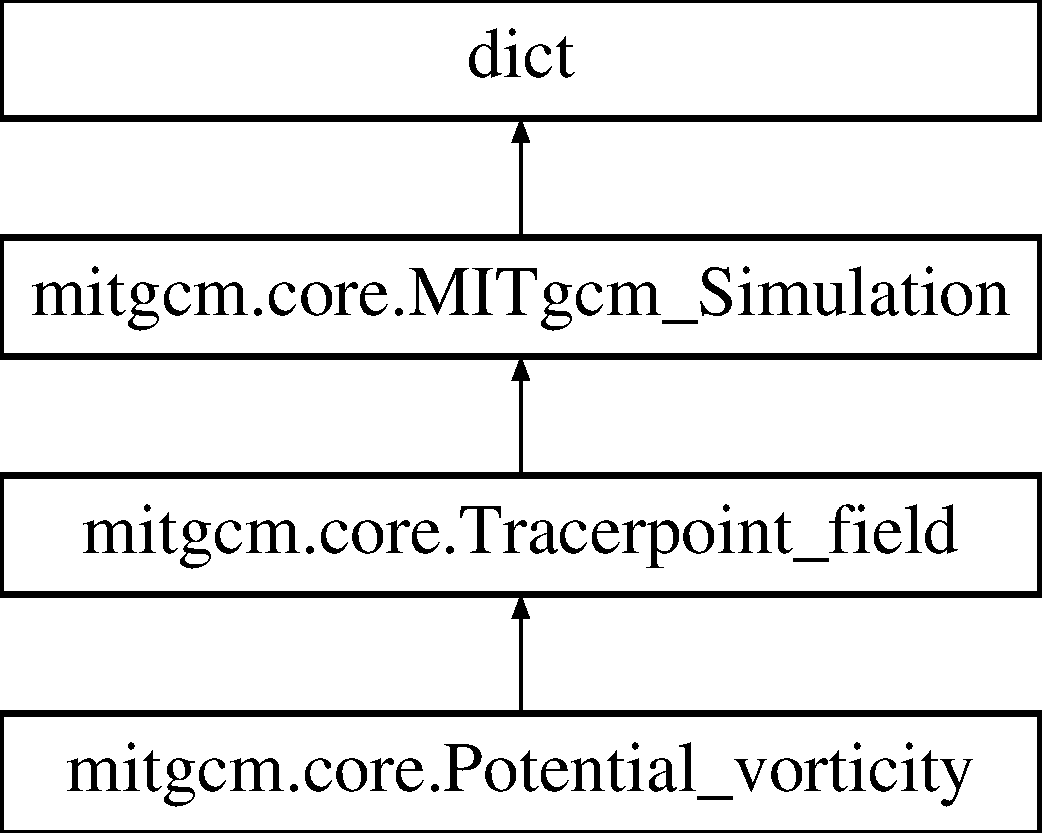
\includegraphics[height=4.000000cm]{classmitgcm_1_1core_1_1Potential__vorticity}
\end{center}
\end{figure}
\subsection*{Public Member Functions}
\begin{DoxyCompactItemize}
\item 
def \hyperlink{classmitgcm_1_1core_1_1Potential__vorticity_aa5cd85f4c534241e18601d592c30b098}{\+\_\+\+\_\+init\+\_\+\+\_\+}
\end{DoxyCompactItemize}
\subsection*{Additional Inherited Members}


\subsection{Detailed Description}
Evaluate the potential vorticity on the tracer points. 



Definition at line 720 of file core.\+py.



\subsection{Constructor \& Destructor Documentation}
\hypertarget{classmitgcm_1_1core_1_1Potential__vorticity_aa5cd85f4c534241e18601d592c30b098}{\index{mitgcm\+::core\+::\+Potential\+\_\+vorticity@{mitgcm\+::core\+::\+Potential\+\_\+vorticity}!\+\_\+\+\_\+init\+\_\+\+\_\+@{\+\_\+\+\_\+init\+\_\+\+\_\+}}
\index{\+\_\+\+\_\+init\+\_\+\+\_\+@{\+\_\+\+\_\+init\+\_\+\+\_\+}!mitgcm\+::core\+::\+Potential\+\_\+vorticity@{mitgcm\+::core\+::\+Potential\+\_\+vorticity}}
\subsubsection[{\+\_\+\+\_\+init\+\_\+\+\_\+}]{\setlength{\rightskip}{0pt plus 5cm}def mitgcm.\+core.\+Potential\+\_\+vorticity.\+\_\+\+\_\+init\+\_\+\+\_\+ (
\begin{DoxyParamCaption}
\item[{}]{self, }
\item[{}]{model\+\_\+instance}
\end{DoxyParamCaption}
)}}\label{classmitgcm_1_1core_1_1Potential__vorticity_aa5cd85f4c534241e18601d592c30b098}


Definition at line 721 of file core.\+py.



The documentation for this class was generated from the following file\+:\begin{DoxyCompactItemize}
\item 
\hyperlink{core_8py}{core.\+py}\end{DoxyCompactItemize}

\hypertarget{classmitgcm_1_1core_1_1Pressure}{\section{mitgcm.\+core.\+Pressure Class Reference}
\label{classmitgcm_1_1core_1_1Pressure}\index{mitgcm.\+core.\+Pressure@{mitgcm.\+core.\+Pressure}}
}
Inheritance diagram for mitgcm.\+core.\+Pressure\+:\begin{figure}[H]
\begin{center}
\leavevmode
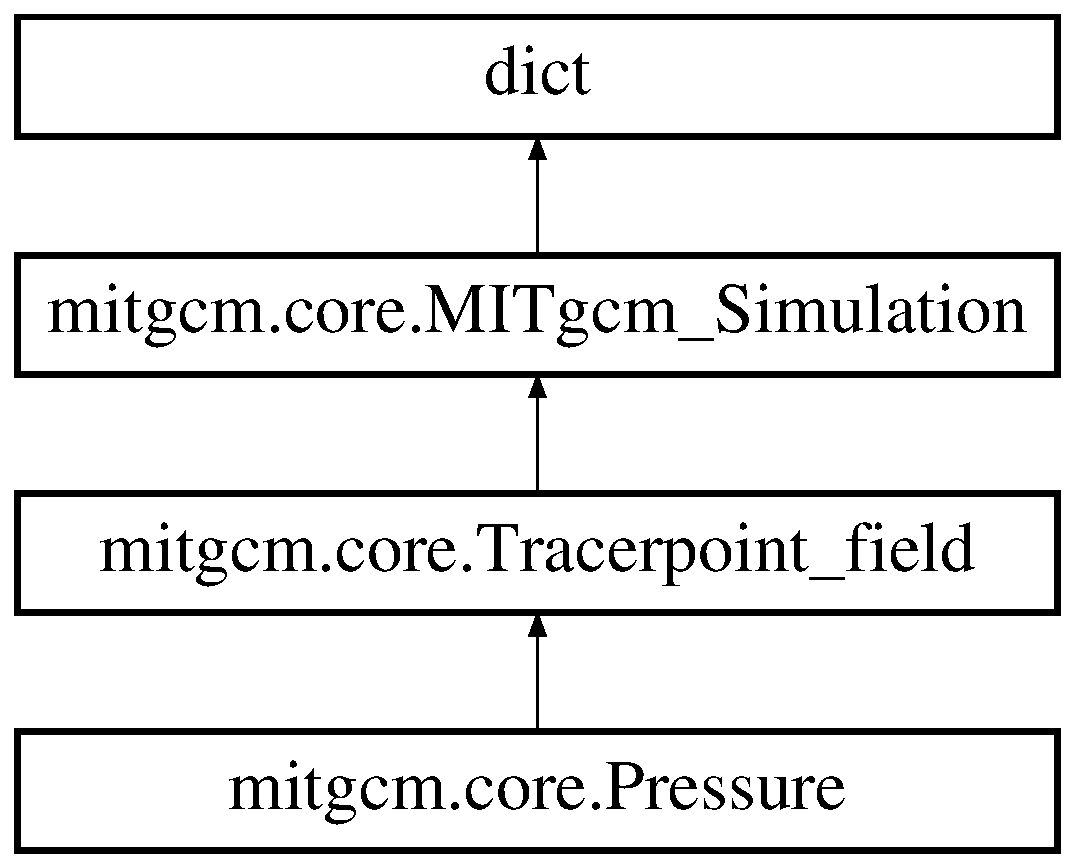
\includegraphics[height=4.000000cm]{classmitgcm_1_1core_1_1Pressure}
\end{center}
\end{figure}
\subsection*{Public Member Functions}
\begin{DoxyCompactItemize}
\item 
def \hyperlink{classmitgcm_1_1core_1_1Pressure_a015248e433a994b90e08ec3123687ec8}{\+\_\+\+\_\+init\+\_\+\+\_\+}
\end{DoxyCompactItemize}
\subsection*{Additional Inherited Members}


\subsection{Detailed Description}


Definition at line 695 of file core.\+py.



\subsection{Constructor \& Destructor Documentation}
\hypertarget{classmitgcm_1_1core_1_1Pressure_a015248e433a994b90e08ec3123687ec8}{\index{mitgcm\+::core\+::\+Pressure@{mitgcm\+::core\+::\+Pressure}!\+\_\+\+\_\+init\+\_\+\+\_\+@{\+\_\+\+\_\+init\+\_\+\+\_\+}}
\index{\+\_\+\+\_\+init\+\_\+\+\_\+@{\+\_\+\+\_\+init\+\_\+\+\_\+}!mitgcm\+::core\+::\+Pressure@{mitgcm\+::core\+::\+Pressure}}
\subsubsection[{\+\_\+\+\_\+init\+\_\+\+\_\+}]{\setlength{\rightskip}{0pt plus 5cm}def mitgcm.\+core.\+Pressure.\+\_\+\+\_\+init\+\_\+\+\_\+ (
\begin{DoxyParamCaption}
\item[{}]{self, }
\item[{}]{model\+\_\+instance}
\end{DoxyParamCaption}
)}}\label{classmitgcm_1_1core_1_1Pressure_a015248e433a994b90e08ec3123687ec8}


Definition at line 696 of file core.\+py.



The documentation for this class was generated from the following file\+:\begin{DoxyCompactItemize}
\item 
\hyperlink{core_8py}{core.\+py}\end{DoxyCompactItemize}

\hypertarget{classmitgcm_1_1core_1_1Temperature}{\section{mitgcm.\+core.\+Temperature Class Reference}
\label{classmitgcm_1_1core_1_1Temperature}\index{mitgcm.\+core.\+Temperature@{mitgcm.\+core.\+Temperature}}
}
Inheritance diagram for mitgcm.\+core.\+Temperature\+:\begin{figure}[H]
\begin{center}
\leavevmode
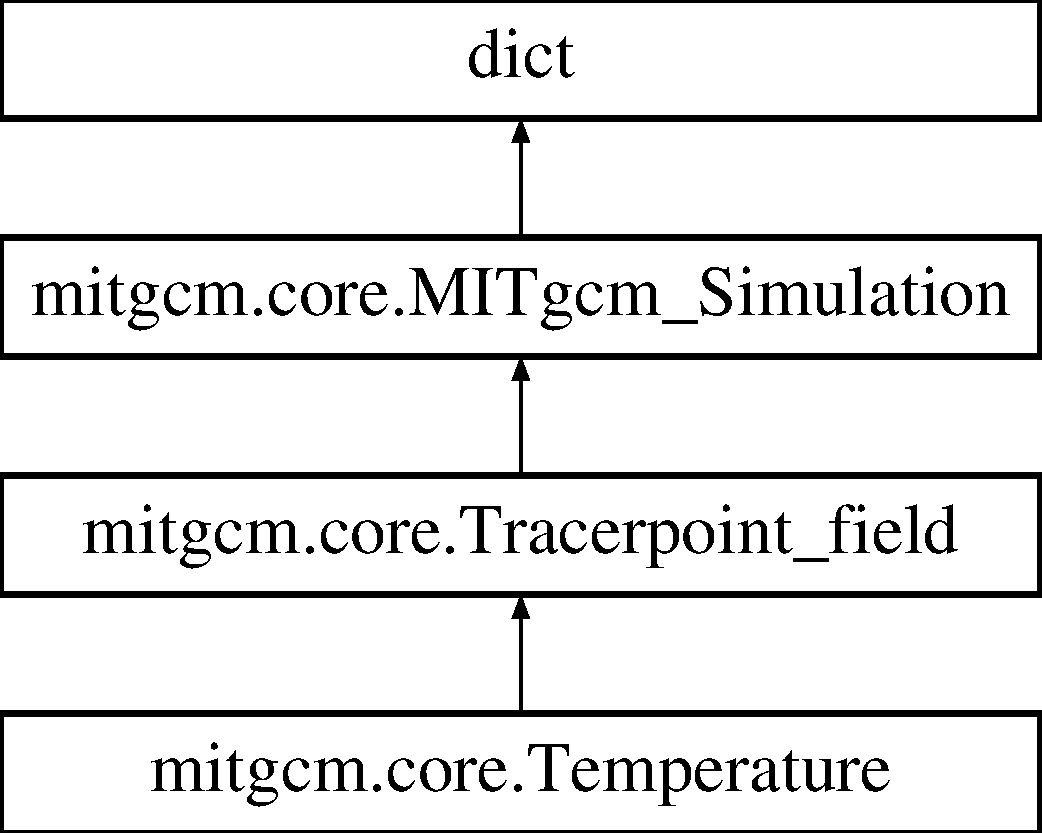
\includegraphics[height=4.000000cm]{classmitgcm_1_1core_1_1Temperature}
\end{center}
\end{figure}
\subsection*{Public Member Functions}
\begin{DoxyCompactItemize}
\item 
def \hyperlink{classmitgcm_1_1core_1_1Temperature_afd2f12d54ed18890fe7117d24c9c3da7}{\+\_\+\+\_\+init\+\_\+\+\_\+}
\end{DoxyCompactItemize}
\subsection*{Additional Inherited Members}


\subsection{Detailed Description}


Definition at line 632 of file core.\+py.



\subsection{Constructor \& Destructor Documentation}
\hypertarget{classmitgcm_1_1core_1_1Temperature_afd2f12d54ed18890fe7117d24c9c3da7}{\index{mitgcm\+::core\+::\+Temperature@{mitgcm\+::core\+::\+Temperature}!\+\_\+\+\_\+init\+\_\+\+\_\+@{\+\_\+\+\_\+init\+\_\+\+\_\+}}
\index{\+\_\+\+\_\+init\+\_\+\+\_\+@{\+\_\+\+\_\+init\+\_\+\+\_\+}!mitgcm\+::core\+::\+Temperature@{mitgcm\+::core\+::\+Temperature}}
\subsubsection[{\+\_\+\+\_\+init\+\_\+\+\_\+}]{\setlength{\rightskip}{0pt plus 5cm}def mitgcm.\+core.\+Temperature.\+\_\+\+\_\+init\+\_\+\+\_\+ (
\begin{DoxyParamCaption}
\item[{}]{self, }
\item[{}]{netcdf\+\_\+filename, }
\item[{}]{variable, }
\item[{}]{time\+\_\+level}
\end{DoxyParamCaption}
)}}\label{classmitgcm_1_1core_1_1Temperature_afd2f12d54ed18890fe7117d24c9c3da7}


Definition at line 633 of file core.\+py.



The documentation for this class was generated from the following file\+:\begin{DoxyCompactItemize}
\item 
\hyperlink{core_8py}{core.\+py}\end{DoxyCompactItemize}

\hypertarget{classmitgcm_1_1core_1_1Tracerpoint__field}{\section{mitgcm.\+core.\+Tracerpoint\+\_\+field Class Reference}
\label{classmitgcm_1_1core_1_1Tracerpoint__field}\index{mitgcm.\+core.\+Tracerpoint\+\_\+field@{mitgcm.\+core.\+Tracerpoint\+\_\+field}}
}


This is the base class for all model fields on the tracer points.  


Inheritance diagram for mitgcm.\+core.\+Tracerpoint\+\_\+field\+:\begin{figure}[H]
\begin{center}
\leavevmode
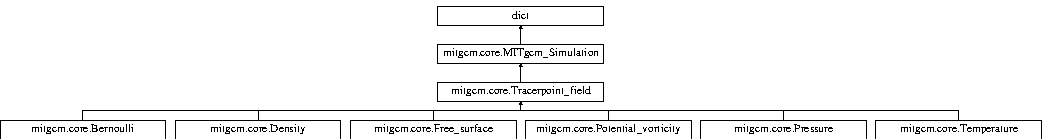
\includegraphics[height=1.866667cm]{classmitgcm_1_1core_1_1Tracerpoint__field}
\end{center}
\end{figure}
\subsection*{Public Member Functions}
\begin{DoxyCompactItemize}
\item 
def \hyperlink{classmitgcm_1_1core_1_1Tracerpoint__field_a4e5ca6800530f2c8da4bc3d21ef4e50d}{take\+\_\+d\+\_\+dx}
\begin{DoxyCompactList}\small\item\em Take the x derivative of the field on tracer points, using spacings in grid object. \end{DoxyCompactList}\item 
def \hyperlink{classmitgcm_1_1core_1_1Tracerpoint__field_a5292f8f5c2110f476329806bee9315bf}{take\+\_\+d\+\_\+dy}
\begin{DoxyCompactList}\small\item\em Take the y derivative of the field on tracer points, using spacings in grid object. \end{DoxyCompactList}\item 
def \hyperlink{classmitgcm_1_1core_1_1Tracerpoint__field_aa54bc7f1fe31f946b3ed13cc1c66f22e}{take\+\_\+d\+\_\+dz}
\begin{DoxyCompactList}\small\item\em Take the z derivative of the field given on tracer-\/points, using the spacings in grid object. \end{DoxyCompactList}\end{DoxyCompactItemize}
\subsection*{Additional Inherited Members}


\subsection{Detailed Description}
This is the base class for all model fields on the tracer points. 

It includes definitions for taking derivatives. 

Definition at line 464 of file core.\+py.



\subsection{Member Function Documentation}
\hypertarget{classmitgcm_1_1core_1_1Tracerpoint__field_a4e5ca6800530f2c8da4bc3d21ef4e50d}{\index{mitgcm\+::core\+::\+Tracerpoint\+\_\+field@{mitgcm\+::core\+::\+Tracerpoint\+\_\+field}!take\+\_\+d\+\_\+dx@{take\+\_\+d\+\_\+dx}}
\index{take\+\_\+d\+\_\+dx@{take\+\_\+d\+\_\+dx}!mitgcm\+::core\+::\+Tracerpoint\+\_\+field@{mitgcm\+::core\+::\+Tracerpoint\+\_\+field}}
\subsubsection[{take\+\_\+d\+\_\+dx}]{\setlength{\rightskip}{0pt plus 5cm}def mitgcm.\+core.\+Tracerpoint\+\_\+field.\+take\+\_\+d\+\_\+dx (
\begin{DoxyParamCaption}
\item[{}]{self, }
\item[{}]{model\+\_\+instance, }
\item[{}]{input\+\_\+field = {\ttfamily 'RHO'}, }
\item[{}]{output\+\_\+field = {\ttfamily 'dRHO\+\_\+dx'}}
\end{DoxyParamCaption}
)}}\label{classmitgcm_1_1core_1_1Tracerpoint__field_a4e5ca6800530f2c8da4bc3d21ef4e50d}


Take the x derivative of the field on tracer points, using spacings in grid object. 

Performs centred second-\/order differencing everywhere except next to boundaries. First order is used there (meaning the gradients at the boundary are evaluated half a grid point away from where they should be). 

Definition at line 472 of file core.\+py.

\hypertarget{classmitgcm_1_1core_1_1Tracerpoint__field_a5292f8f5c2110f476329806bee9315bf}{\index{mitgcm\+::core\+::\+Tracerpoint\+\_\+field@{mitgcm\+::core\+::\+Tracerpoint\+\_\+field}!take\+\_\+d\+\_\+dy@{take\+\_\+d\+\_\+dy}}
\index{take\+\_\+d\+\_\+dy@{take\+\_\+d\+\_\+dy}!mitgcm\+::core\+::\+Tracerpoint\+\_\+field@{mitgcm\+::core\+::\+Tracerpoint\+\_\+field}}
\subsubsection[{take\+\_\+d\+\_\+dy}]{\setlength{\rightskip}{0pt plus 5cm}def mitgcm.\+core.\+Tracerpoint\+\_\+field.\+take\+\_\+d\+\_\+dy (
\begin{DoxyParamCaption}
\item[{}]{self, }
\item[{}]{model\+\_\+instance, }
\item[{}]{input\+\_\+field = {\ttfamily 'RHO'}, }
\item[{}]{output\+\_\+field = {\ttfamily 'dRHO\+\_\+dy'}}
\end{DoxyParamCaption}
)}}\label{classmitgcm_1_1core_1_1Tracerpoint__field_a5292f8f5c2110f476329806bee9315bf}


Take the y derivative of the field on tracer points, using spacings in grid object. 

Performs centred second-\/order differencing everywhere except next to boundaries. First order is used there (meaning the gradients at the boundary are evaluated half a grid point away from where they should be). 

Definition at line 504 of file core.\+py.

\hypertarget{classmitgcm_1_1core_1_1Tracerpoint__field_aa54bc7f1fe31f946b3ed13cc1c66f22e}{\index{mitgcm\+::core\+::\+Tracerpoint\+\_\+field@{mitgcm\+::core\+::\+Tracerpoint\+\_\+field}!take\+\_\+d\+\_\+dz@{take\+\_\+d\+\_\+dz}}
\index{take\+\_\+d\+\_\+dz@{take\+\_\+d\+\_\+dz}!mitgcm\+::core\+::\+Tracerpoint\+\_\+field@{mitgcm\+::core\+::\+Tracerpoint\+\_\+field}}
\subsubsection[{take\+\_\+d\+\_\+dz}]{\setlength{\rightskip}{0pt plus 5cm}def mitgcm.\+core.\+Tracerpoint\+\_\+field.\+take\+\_\+d\+\_\+dz (
\begin{DoxyParamCaption}
\item[{}]{self, }
\item[{}]{model\+\_\+instance, }
\item[{}]{input\+\_\+field = {\ttfamily 'RHO'}, }
\item[{}]{output\+\_\+field = {\ttfamily 'dRHO\+\_\+dz'}}
\end{DoxyParamCaption}
)}}\label{classmitgcm_1_1core_1_1Tracerpoint__field_aa54bc7f1fe31f946b3ed13cc1c66f22e}


Take the z derivative of the field given on tracer-\/points, using the spacings in grid object. 

Performs centred second-\/order differencing everywhere except next to boundaries. First order is used there (meaning the gradients at the boundary are evaluated half a grid point away from where they should be). 

Definition at line 536 of file core.\+py.



The documentation for this class was generated from the following file\+:\begin{DoxyCompactItemize}
\item 
\hyperlink{core_8py}{core.\+py}\end{DoxyCompactItemize}

\hypertarget{classmitgcm_1_1core_1_1Upoint__field}{}\section{mitgcm.\+core.\+Upoint\+\_\+field Class Reference}
\label{classmitgcm_1_1core_1_1Upoint__field}\index{mitgcm.\+core.\+Upoint\+\_\+field@{mitgcm.\+core.\+Upoint\+\_\+field}}


This is the class for all fields on zonal velocity points.  


Inheritance diagram for mitgcm.\+core.\+Upoint\+\_\+field\+:\begin{figure}[H]
\begin{center}
\leavevmode
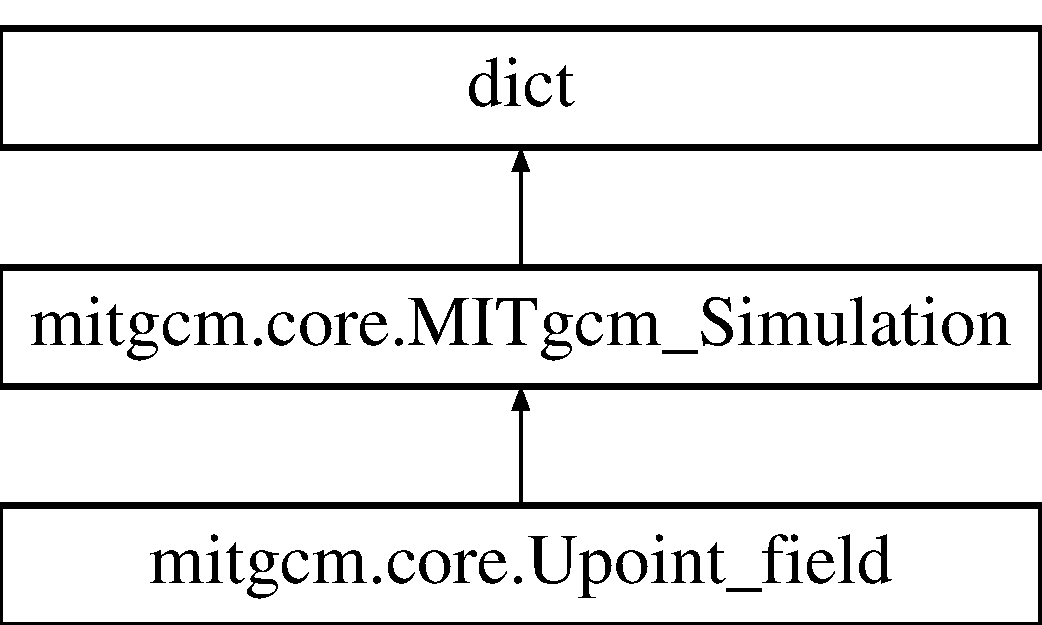
\includegraphics[height=3.000000cm]{classmitgcm_1_1core_1_1Upoint__field}
\end{center}
\end{figure}
\subsection*{Public Member Functions}
\begin{DoxyCompactItemize}
\item 
def \hyperlink{classmitgcm_1_1core_1_1Upoint__field_ab4adbcfd61c7b303b8499a5228cd6f77}{\+\_\+\+\_\+init\+\_\+\+\_\+}
\item 
def \hyperlink{classmitgcm_1_1core_1_1Upoint__field_a40c4ea3c2527688e8419c0a276e27d5c}{take\+\_\+d\+\_\+dx}
\begin{DoxyCompactList}\small\item\em Derivatives of model fields. \end{DoxyCompactList}\item 
def \hyperlink{classmitgcm_1_1core_1_1Upoint__field_acac1cef0245cd27c0975a84bef22a71d}{take\+\_\+d\+\_\+dy}
\begin{DoxyCompactList}\small\item\em Take the y derivative of the field on u points, using the spacings provided. \end{DoxyCompactList}\item 
def \hyperlink{classmitgcm_1_1core_1_1Upoint__field_acbc550b512401054ac04eca3dc7318af}{take\+\_\+d\+\_\+dz}
\begin{DoxyCompactList}\small\item\em Take the z derivative of the field given on u-\/points, using the spacings in grid object. \end{DoxyCompactList}\end{DoxyCompactItemize}
\subsection*{Additional Inherited Members}


\subsection{Detailed Description}
This is the class for all fields on zonal velocity points. 



Definition at line 103 of file core.\+py.



\subsection{Constructor \& Destructor Documentation}
\hypertarget{classmitgcm_1_1core_1_1Upoint__field_ab4adbcfd61c7b303b8499a5228cd6f77}{}\index{mitgcm\+::core\+::\+Upoint\+\_\+field@{mitgcm\+::core\+::\+Upoint\+\_\+field}!\+\_\+\+\_\+init\+\_\+\+\_\+@{\+\_\+\+\_\+init\+\_\+\+\_\+}}
\index{\+\_\+\+\_\+init\+\_\+\+\_\+@{\+\_\+\+\_\+init\+\_\+\+\_\+}!mitgcm\+::core\+::\+Upoint\+\_\+field@{mitgcm\+::core\+::\+Upoint\+\_\+field}}
\subsubsection[{\+\_\+\+\_\+init\+\_\+\+\_\+}]{\setlength{\rightskip}{0pt plus 5cm}def mitgcm.\+core.\+Upoint\+\_\+field.\+\_\+\+\_\+init\+\_\+\+\_\+ (
\begin{DoxyParamCaption}
\item[{}]{self, }
\item[{}]{netcdf\+\_\+filename, }
\item[{}]{variable, }
\item[{}]{time\+\_\+level, }
\item[{}]{empty = {\ttfamily False}}
\end{DoxyParamCaption}
)}\label{classmitgcm_1_1core_1_1Upoint__field_ab4adbcfd61c7b303b8499a5228cd6f77}


Definition at line 105 of file core.\+py.



\subsection{Member Function Documentation}
\hypertarget{classmitgcm_1_1core_1_1Upoint__field_a40c4ea3c2527688e8419c0a276e27d5c}{}\index{mitgcm\+::core\+::\+Upoint\+\_\+field@{mitgcm\+::core\+::\+Upoint\+\_\+field}!take\+\_\+d\+\_\+dx@{take\+\_\+d\+\_\+dx}}
\index{take\+\_\+d\+\_\+dx@{take\+\_\+d\+\_\+dx}!mitgcm\+::core\+::\+Upoint\+\_\+field@{mitgcm\+::core\+::\+Upoint\+\_\+field}}
\subsubsection[{take\+\_\+d\+\_\+dx}]{\setlength{\rightskip}{0pt plus 5cm}def mitgcm.\+core.\+Upoint\+\_\+field.\+take\+\_\+d\+\_\+dx (
\begin{DoxyParamCaption}
\item[{}]{self, }
\item[{}]{model\+\_\+instance, }
\item[{}]{input\+\_\+field = {\ttfamily \textquotesingle{}UVEL\textquotesingle{}}, }
\item[{}]{output\+\_\+field = {\ttfamily \textquotesingle{}dU\+\_\+dx\textquotesingle{}}}
\end{DoxyParamCaption}
)}\label{classmitgcm_1_1core_1_1Upoint__field_a40c4ea3c2527688e8419c0a276e27d5c}


Derivatives of model fields. 

Take the x derivative of the field given on u-\/points, using the spacings in grid object. \begin{DoxyVerb}   Performs centred second-order differencing everywhere except next to boundaries. First order is 
   used there (meaning the gradients at the boundary are evaluated half a grid point away from where 
   they should be). \end{DoxyVerb}
 

Definition at line 120 of file core.\+py.

\hypertarget{classmitgcm_1_1core_1_1Upoint__field_acac1cef0245cd27c0975a84bef22a71d}{}\index{mitgcm\+::core\+::\+Upoint\+\_\+field@{mitgcm\+::core\+::\+Upoint\+\_\+field}!take\+\_\+d\+\_\+dy@{take\+\_\+d\+\_\+dy}}
\index{take\+\_\+d\+\_\+dy@{take\+\_\+d\+\_\+dy}!mitgcm\+::core\+::\+Upoint\+\_\+field@{mitgcm\+::core\+::\+Upoint\+\_\+field}}
\subsubsection[{take\+\_\+d\+\_\+dy}]{\setlength{\rightskip}{0pt plus 5cm}def mitgcm.\+core.\+Upoint\+\_\+field.\+take\+\_\+d\+\_\+dy (
\begin{DoxyParamCaption}
\item[{}]{self, }
\item[{}]{model\+\_\+instance, }
\item[{}]{input\+\_\+field = {\ttfamily \textquotesingle{}UVEL\textquotesingle{}}, }
\item[{}]{output\+\_\+field = {\ttfamily \textquotesingle{}dU\+\_\+dy\textquotesingle{}}}
\end{DoxyParamCaption}
)}\label{classmitgcm_1_1core_1_1Upoint__field_acac1cef0245cd27c0975a84bef22a71d}


Take the y derivative of the field on u points, using the spacings provided. 

Performs centred second-\/order differencing everywhere except next to boundaries. First order is used there (meaning the gradients at the boundary are evaluated half a grid point away from where they should be). 

Definition at line 156 of file core.\+py.

\hypertarget{classmitgcm_1_1core_1_1Upoint__field_acbc550b512401054ac04eca3dc7318af}{}\index{mitgcm\+::core\+::\+Upoint\+\_\+field@{mitgcm\+::core\+::\+Upoint\+\_\+field}!take\+\_\+d\+\_\+dz@{take\+\_\+d\+\_\+dz}}
\index{take\+\_\+d\+\_\+dz@{take\+\_\+d\+\_\+dz}!mitgcm\+::core\+::\+Upoint\+\_\+field@{mitgcm\+::core\+::\+Upoint\+\_\+field}}
\subsubsection[{take\+\_\+d\+\_\+dz}]{\setlength{\rightskip}{0pt plus 5cm}def mitgcm.\+core.\+Upoint\+\_\+field.\+take\+\_\+d\+\_\+dz (
\begin{DoxyParamCaption}
\item[{}]{self, }
\item[{}]{model\+\_\+instance, }
\item[{}]{input\+\_\+field = {\ttfamily \textquotesingle{}UVEL\textquotesingle{}}, }
\item[{}]{output\+\_\+field = {\ttfamily \textquotesingle{}dU\+\_\+dz\textquotesingle{}}}
\end{DoxyParamCaption}
)}\label{classmitgcm_1_1core_1_1Upoint__field_acbc550b512401054ac04eca3dc7318af}


Take the z derivative of the field given on u-\/points, using the spacings in grid object. 

Performs centred second-\/order differencing everywhere except next to boundaries. First order is used there (meaning the gradients at the boundary are evaluated half a grid point away from where they should be). 

Definition at line 193 of file core.\+py.



The documentation for this class was generated from the following file\+:\begin{DoxyCompactItemize}
\item 
\hyperlink{core_8py}{core.\+py}\end{DoxyCompactItemize}

\hypertarget{classmitgcm_1_1core_1_1Vorticity}{\section{mitgcm.\+core.\+Vorticity Class Reference}
\label{classmitgcm_1_1core_1_1Vorticity}\index{mitgcm.\+core.\+Vorticity@{mitgcm.\+core.\+Vorticity}}
}
Inheritance diagram for mitgcm.\+core.\+Vorticity\+:\begin{figure}[H]
\begin{center}
\leavevmode
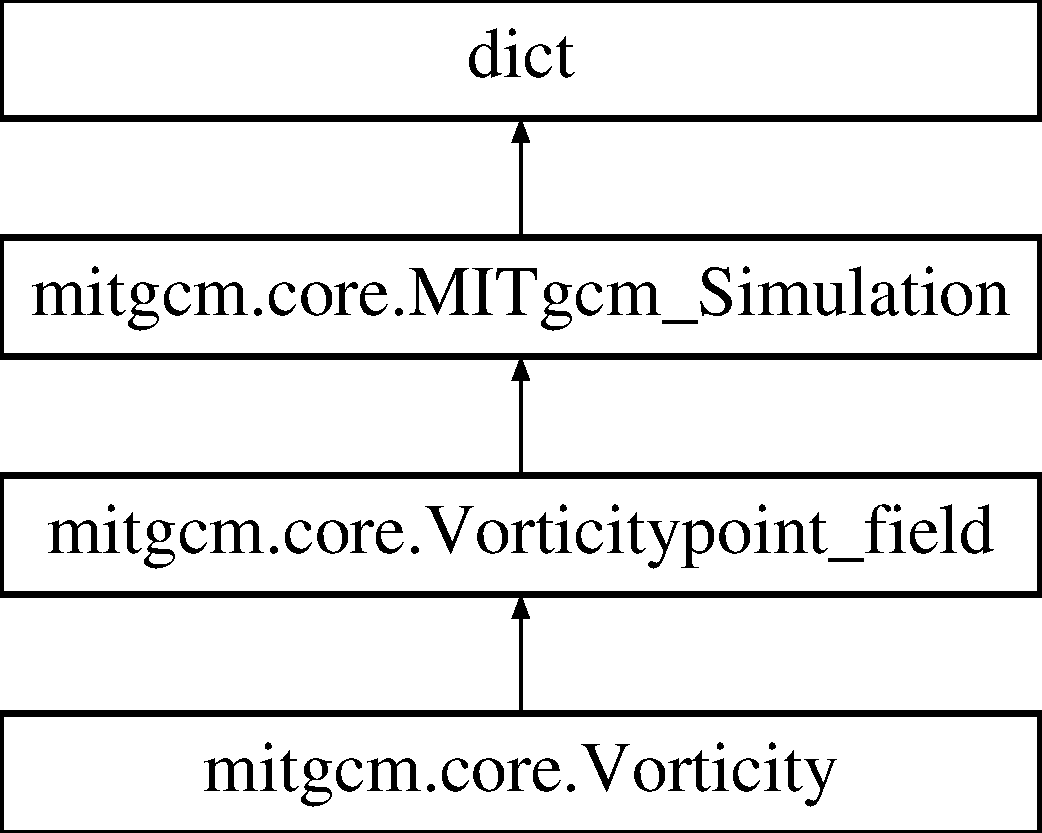
\includegraphics[height=4.000000cm]{classmitgcm_1_1core_1_1Vorticity}
\end{center}
\end{figure}
\subsection*{Public Member Functions}
\begin{DoxyCompactItemize}
\item 
def \hyperlink{classmitgcm_1_1core_1_1Vorticity_a43bff58c89253c8425aef49b7ab37e2d}{\+\_\+\+\_\+init\+\_\+\+\_\+}
\end{DoxyCompactItemize}
\subsection*{Additional Inherited Members}


\subsection{Detailed Description}


Definition at line 743 of file core.\+py.



\subsection{Constructor \& Destructor Documentation}
\hypertarget{classmitgcm_1_1core_1_1Vorticity_a43bff58c89253c8425aef49b7ab37e2d}{\index{mitgcm\+::core\+::\+Vorticity@{mitgcm\+::core\+::\+Vorticity}!\+\_\+\+\_\+init\+\_\+\+\_\+@{\+\_\+\+\_\+init\+\_\+\+\_\+}}
\index{\+\_\+\+\_\+init\+\_\+\+\_\+@{\+\_\+\+\_\+init\+\_\+\+\_\+}!mitgcm\+::core\+::\+Vorticity@{mitgcm\+::core\+::\+Vorticity}}
\subsubsection[{\+\_\+\+\_\+init\+\_\+\+\_\+}]{\setlength{\rightskip}{0pt plus 5cm}def mitgcm.\+core.\+Vorticity.\+\_\+\+\_\+init\+\_\+\+\_\+ (
\begin{DoxyParamCaption}
\item[{}]{self, }
\item[{}]{netcdf\+\_\+filename = {\ttfamily '3D\+\_\+fields.all.nc'}, }
\item[{}]{variable = {\ttfamily 'momVort3'}, }
\item[{}]{time\+\_\+level = {\ttfamily 0}, }
\item[{}]{empty = {\ttfamily False}}
\end{DoxyParamCaption}
)}}\label{classmitgcm_1_1core_1_1Vorticity_a43bff58c89253c8425aef49b7ab37e2d}


Definition at line 744 of file core.\+py.



The documentation for this class was generated from the following file\+:\begin{DoxyCompactItemize}
\item 
\hyperlink{core_8py}{core.\+py}\end{DoxyCompactItemize}

\hypertarget{classmitgcm_1_1core_1_1Vorticitypoint__field}{\section{mitgcm.\+core.\+Vorticitypoint\+\_\+field Class Reference}
\label{classmitgcm_1_1core_1_1Vorticitypoint__field}\index{mitgcm.\+core.\+Vorticitypoint\+\_\+field@{mitgcm.\+core.\+Vorticitypoint\+\_\+field}}
}
Inheritance diagram for mitgcm.\+core.\+Vorticitypoint\+\_\+field\+:\begin{figure}[H]
\begin{center}
\leavevmode
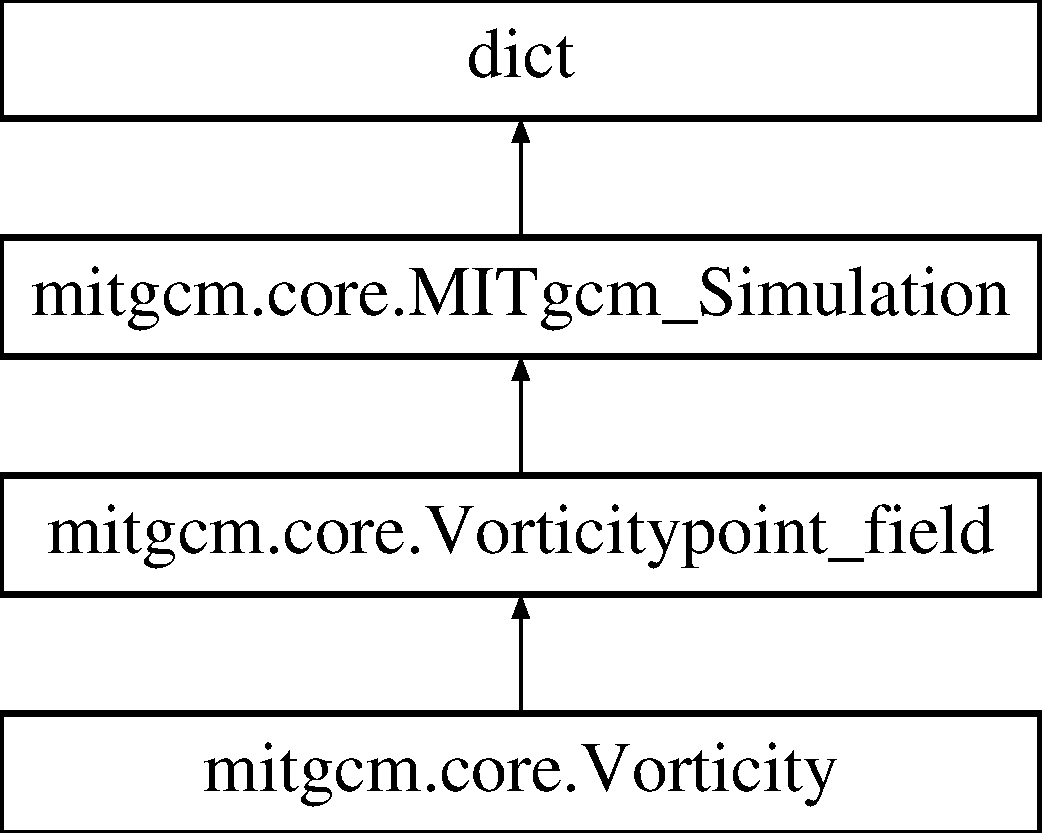
\includegraphics[height=4.000000cm]{classmitgcm_1_1core_1_1Vorticitypoint__field}
\end{center}
\end{figure}
\subsection*{Additional Inherited Members}


\subsection{Detailed Description}


Definition at line 537 of file core.\+py.



The documentation for this class was generated from the following file\+:\begin{DoxyCompactItemize}
\item 
\hyperlink{core_8py}{core.\+py}\end{DoxyCompactItemize}

\hypertarget{classmitgcm_1_1core_1_1Vpoint__field}{\section{mitgcm.\+core.\+Vpoint\+\_\+field Class Reference}
\label{classmitgcm_1_1core_1_1Vpoint__field}\index{mitgcm.\+core.\+Vpoint\+\_\+field@{mitgcm.\+core.\+Vpoint\+\_\+field}}
}


This is the class fo rall fields on meridional velocity points.  


Inheritance diagram for mitgcm.\+core.\+Vpoint\+\_\+field\+:\begin{figure}[H]
\begin{center}
\leavevmode
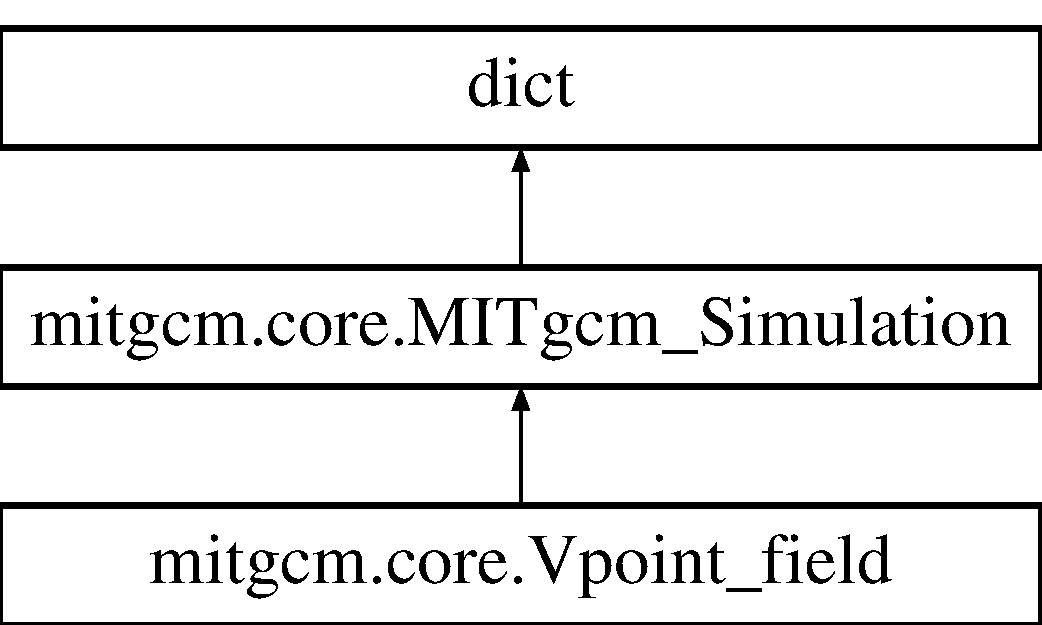
\includegraphics[height=3.000000cm]{classmitgcm_1_1core_1_1Vpoint__field}
\end{center}
\end{figure}
\subsection*{Public Member Functions}
\begin{DoxyCompactItemize}
\item 
def \hyperlink{classmitgcm_1_1core_1_1Vpoint__field_a1ffd906684a51a4045b0b02092fab5ec}{\+\_\+\+\_\+init\+\_\+\+\_\+}
\begin{DoxyCompactList}\small\item\em Instantiate a field on the meridional velocity points. \end{DoxyCompactList}\item 
def \hyperlink{classmitgcm_1_1core_1_1Vpoint__field_a0077d0cdd01de210b130f1e684d61b6d}{take\+\_\+d\+\_\+dx}
\begin{DoxyCompactList}\small\item\em Take the x derivative of the field on v points using the spacings in model\+\_\+instance.\+grid object. \end{DoxyCompactList}\item 
def \hyperlink{classmitgcm_1_1core_1_1Vpoint__field_a7ffa6c1b239c78422f0224d675fd785e}{take\+\_\+d\+\_\+dy}
\begin{DoxyCompactList}\small\item\em Take the y derivative of the field given on v-\/points, using the spacings in grid object. \end{DoxyCompactList}\item 
def \hyperlink{classmitgcm_1_1core_1_1Vpoint__field_a9975d2dcfb23b8cca0986f7e469882fa}{take\+\_\+d\+\_\+dz}
\begin{DoxyCompactList}\small\item\em Take the z derivative of the field given on v-\/points, using the spacings in grid object. \end{DoxyCompactList}\end{DoxyCompactItemize}
\subsection*{Additional Inherited Members}


\subsection{Detailed Description}
This is the class fo rall fields on meridional velocity points. 



Definition at line 206 of file core.\+py.



\subsection{Constructor \& Destructor Documentation}
\hypertarget{classmitgcm_1_1core_1_1Vpoint__field_a1ffd906684a51a4045b0b02092fab5ec}{\index{mitgcm\+::core\+::\+Vpoint\+\_\+field@{mitgcm\+::core\+::\+Vpoint\+\_\+field}!\+\_\+\+\_\+init\+\_\+\+\_\+@{\+\_\+\+\_\+init\+\_\+\+\_\+}}
\index{\+\_\+\+\_\+init\+\_\+\+\_\+@{\+\_\+\+\_\+init\+\_\+\+\_\+}!mitgcm\+::core\+::\+Vpoint\+\_\+field@{mitgcm\+::core\+::\+Vpoint\+\_\+field}}
\subsubsection[{\+\_\+\+\_\+init\+\_\+\+\_\+}]{\setlength{\rightskip}{0pt plus 5cm}def mitgcm.\+core.\+Vpoint\+\_\+field.\+\_\+\+\_\+init\+\_\+\+\_\+ (
\begin{DoxyParamCaption}
\item[{}]{self, }
\item[{}]{netcdf\+\_\+filename, }
\item[{}]{variable, }
\item[{}]{time\+\_\+level}
\end{DoxyParamCaption}
)}}\label{classmitgcm_1_1core_1_1Vpoint__field_a1ffd906684a51a4045b0b02092fab5ec}


Instantiate a field on the meridional velocity points. 



Definition at line 210 of file core.\+py.



\subsection{Member Function Documentation}
\hypertarget{classmitgcm_1_1core_1_1Vpoint__field_a0077d0cdd01de210b130f1e684d61b6d}{\index{mitgcm\+::core\+::\+Vpoint\+\_\+field@{mitgcm\+::core\+::\+Vpoint\+\_\+field}!take\+\_\+d\+\_\+dx@{take\+\_\+d\+\_\+dx}}
\index{take\+\_\+d\+\_\+dx@{take\+\_\+d\+\_\+dx}!mitgcm\+::core\+::\+Vpoint\+\_\+field@{mitgcm\+::core\+::\+Vpoint\+\_\+field}}
\subsubsection[{take\+\_\+d\+\_\+dx}]{\setlength{\rightskip}{0pt plus 5cm}def mitgcm.\+core.\+Vpoint\+\_\+field.\+take\+\_\+d\+\_\+dx (
\begin{DoxyParamCaption}
\item[{}]{self, }
\item[{}]{model\+\_\+instance, }
\item[{}]{input\+\_\+field = {\ttfamily 'VVEL'}, }
\item[{}]{output\+\_\+field = {\ttfamily 'dV\+\_\+dx'}}
\end{DoxyParamCaption}
)}}\label{classmitgcm_1_1core_1_1Vpoint__field_a0077d0cdd01de210b130f1e684d61b6d}


Take the x derivative of the field on v points using the spacings in model\+\_\+instance.\+grid object. 

This function can be daisy-\/chained to get higher order derivatives.

Performs centred second-\/order differencing everywhere except next to boundaries. First order is used there (meaning the gradients at the boundary are evaluated half a grid point away from where they should be). 

Definition at line 223 of file core.\+py.

\hypertarget{classmitgcm_1_1core_1_1Vpoint__field_a7ffa6c1b239c78422f0224d675fd785e}{\index{mitgcm\+::core\+::\+Vpoint\+\_\+field@{mitgcm\+::core\+::\+Vpoint\+\_\+field}!take\+\_\+d\+\_\+dy@{take\+\_\+d\+\_\+dy}}
\index{take\+\_\+d\+\_\+dy@{take\+\_\+d\+\_\+dy}!mitgcm\+::core\+::\+Vpoint\+\_\+field@{mitgcm\+::core\+::\+Vpoint\+\_\+field}}
\subsubsection[{take\+\_\+d\+\_\+dy}]{\setlength{\rightskip}{0pt plus 5cm}def mitgcm.\+core.\+Vpoint\+\_\+field.\+take\+\_\+d\+\_\+dy (
\begin{DoxyParamCaption}
\item[{}]{self, }
\item[{}]{model\+\_\+instance, }
\item[{}]{input\+\_\+field = {\ttfamily 'VVEL'}, }
\item[{}]{output\+\_\+field = {\ttfamily 'dV\+\_\+dy'}}
\end{DoxyParamCaption}
)}}\label{classmitgcm_1_1core_1_1Vpoint__field_a7ffa6c1b239c78422f0224d675fd785e}


Take the y derivative of the field given on v-\/points, using the spacings in grid object. 

Performs centred second-\/order differencing everywhere except next to boundaries. First order is used there (meaning the gradients at the boundary are evaluated half a grid point away from where they should be). 

Definition at line 254 of file core.\+py.

\hypertarget{classmitgcm_1_1core_1_1Vpoint__field_a9975d2dcfb23b8cca0986f7e469882fa}{\index{mitgcm\+::core\+::\+Vpoint\+\_\+field@{mitgcm\+::core\+::\+Vpoint\+\_\+field}!take\+\_\+d\+\_\+dz@{take\+\_\+d\+\_\+dz}}
\index{take\+\_\+d\+\_\+dz@{take\+\_\+d\+\_\+dz}!mitgcm\+::core\+::\+Vpoint\+\_\+field@{mitgcm\+::core\+::\+Vpoint\+\_\+field}}
\subsubsection[{take\+\_\+d\+\_\+dz}]{\setlength{\rightskip}{0pt plus 5cm}def mitgcm.\+core.\+Vpoint\+\_\+field.\+take\+\_\+d\+\_\+dz (
\begin{DoxyParamCaption}
\item[{}]{self, }
\item[{}]{model\+\_\+instance, }
\item[{}]{input\+\_\+field = {\ttfamily 'VVEL'}, }
\item[{}]{output\+\_\+field = {\ttfamily 'dV\+\_\+dz'}}
\end{DoxyParamCaption}
)}}\label{classmitgcm_1_1core_1_1Vpoint__field_a9975d2dcfb23b8cca0986f7e469882fa}


Take the z derivative of the field given on v-\/points, using the spacings in grid object. 

Performs centred second-\/order differencing everywhere except next to boundaries. First order is used there (meaning the gradients at the boundary are evaluated half a grid point away from where they should be). 

Definition at line 286 of file core.\+py.



The documentation for this class was generated from the following file\+:\begin{DoxyCompactItemize}
\item 
\hyperlink{core_8py}{core.\+py}\end{DoxyCompactItemize}

\hypertarget{classmitgcm_1_1core_1_1Wpoint__field}{\section{mitgcm.\+core.\+Wpoint\+\_\+field Class Reference}
\label{classmitgcm_1_1core_1_1Wpoint__field}\index{mitgcm.\+core.\+Wpoint\+\_\+field@{mitgcm.\+core.\+Wpoint\+\_\+field}}
}
Inheritance diagram for mitgcm.\+core.\+Wpoint\+\_\+field\+:\begin{figure}[H]
\begin{center}
\leavevmode
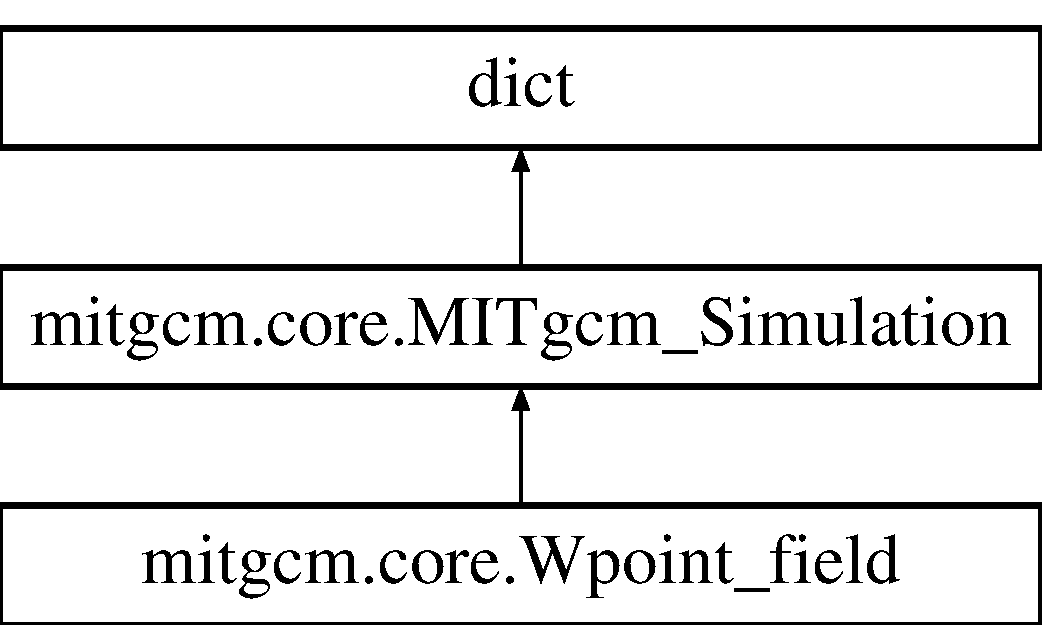
\includegraphics[height=3.000000cm]{classmitgcm_1_1core_1_1Wpoint__field}
\end{center}
\end{figure}
\subsection*{Public Member Functions}
\begin{DoxyCompactItemize}
\item 
def \hyperlink{classmitgcm_1_1core_1_1Wpoint__field_a5149dd8a1c832999bdbcd60b4abc3b14}{\+\_\+\+\_\+init\+\_\+\+\_\+}
\item 
def \hyperlink{classmitgcm_1_1core_1_1Wpoint__field_abc10b27c7fc6fd59b2e525485242d4c1}{load\+\_\+field}
\begin{DoxyCompactList}\small\item\em Load a model field from Net\+C\+D\+F output. \end{DoxyCompactList}\item 
def \hyperlink{classmitgcm_1_1core_1_1Wpoint__field_a3dae400759f1828507a317507dbf681b}{take\+\_\+d\+\_\+dx}
\begin{DoxyCompactList}\small\item\em Take the x derivative of the field on w points, using spacings in grid object. \end{DoxyCompactList}\item 
def \hyperlink{classmitgcm_1_1core_1_1Wpoint__field_a3874bb9811b39ed61b25de3ba3e3c39c}{take\+\_\+d\+\_\+dy}
\begin{DoxyCompactList}\small\item\em Take the y derivative of the field on w points, using spacings in grid object. \end{DoxyCompactList}\item 
def \hyperlink{classmitgcm_1_1core_1_1Wpoint__field_a3f7ffb2f1ed512712805bf78d8a8cde4}{take\+\_\+d\+\_\+dz}
\begin{DoxyCompactList}\small\item\em Take the z derivative of the field given on w-\/points, using the spacings in grid object. \end{DoxyCompactList}\end{DoxyCompactItemize}
\subsection*{Additional Inherited Members}


\subsection{Detailed Description}


Definition at line 310 of file core.\+py.



\subsection{Constructor \& Destructor Documentation}
\hypertarget{classmitgcm_1_1core_1_1Wpoint__field_a5149dd8a1c832999bdbcd60b4abc3b14}{\index{mitgcm\+::core\+::\+Wpoint\+\_\+field@{mitgcm\+::core\+::\+Wpoint\+\_\+field}!\+\_\+\+\_\+init\+\_\+\+\_\+@{\+\_\+\+\_\+init\+\_\+\+\_\+}}
\index{\+\_\+\+\_\+init\+\_\+\+\_\+@{\+\_\+\+\_\+init\+\_\+\+\_\+}!mitgcm\+::core\+::\+Wpoint\+\_\+field@{mitgcm\+::core\+::\+Wpoint\+\_\+field}}
\subsubsection[{\+\_\+\+\_\+init\+\_\+\+\_\+}]{\setlength{\rightskip}{0pt plus 5cm}def mitgcm.\+core.\+Wpoint\+\_\+field.\+\_\+\+\_\+init\+\_\+\+\_\+ (
\begin{DoxyParamCaption}
\item[{}]{self, }
\item[{}]{netcdf\+\_\+filename, }
\item[{}]{variable, }
\item[{}]{time\+\_\+level}
\end{DoxyParamCaption}
)}}\label{classmitgcm_1_1core_1_1Wpoint__field_a5149dd8a1c832999bdbcd60b4abc3b14}


Definition at line 312 of file core.\+py.



\subsection{Member Function Documentation}
\hypertarget{classmitgcm_1_1core_1_1Wpoint__field_abc10b27c7fc6fd59b2e525485242d4c1}{\index{mitgcm\+::core\+::\+Wpoint\+\_\+field@{mitgcm\+::core\+::\+Wpoint\+\_\+field}!load\+\_\+field@{load\+\_\+field}}
\index{load\+\_\+field@{load\+\_\+field}!mitgcm\+::core\+::\+Wpoint\+\_\+field@{mitgcm\+::core\+::\+Wpoint\+\_\+field}}
\subsubsection[{load\+\_\+field}]{\setlength{\rightskip}{0pt plus 5cm}def mitgcm.\+core.\+Wpoint\+\_\+field.\+load\+\_\+field (
\begin{DoxyParamCaption}
\item[{}]{self, }
\item[{}]{netcdf\+\_\+filename, }
\item[{}]{variable, }
\item[{}]{time\+\_\+level}
\end{DoxyParamCaption}
)}}\label{classmitgcm_1_1core_1_1Wpoint__field_abc10b27c7fc6fd59b2e525485242d4c1}


Load a model field from Net\+C\+D\+F output. 

This function associates the field with the object it is called on.

time\+\_\+level can be an integer or an array of integers. If it's an array, then multiple time levels will be returned as a higher dimensional array. 

Definition at line 321 of file core.\+py.

\hypertarget{classmitgcm_1_1core_1_1Wpoint__field_a3dae400759f1828507a317507dbf681b}{\index{mitgcm\+::core\+::\+Wpoint\+\_\+field@{mitgcm\+::core\+::\+Wpoint\+\_\+field}!take\+\_\+d\+\_\+dx@{take\+\_\+d\+\_\+dx}}
\index{take\+\_\+d\+\_\+dx@{take\+\_\+d\+\_\+dx}!mitgcm\+::core\+::\+Wpoint\+\_\+field@{mitgcm\+::core\+::\+Wpoint\+\_\+field}}
\subsubsection[{take\+\_\+d\+\_\+dx}]{\setlength{\rightskip}{0pt plus 5cm}def mitgcm.\+core.\+Wpoint\+\_\+field.\+take\+\_\+d\+\_\+dx (
\begin{DoxyParamCaption}
\item[{}]{self, }
\item[{}]{model\+\_\+instance, }
\item[{}]{input\+\_\+field = {\ttfamily 'WVEL'}, }
\item[{}]{output\+\_\+field = {\ttfamily 'dW\+\_\+dx'}}
\end{DoxyParamCaption}
)}}\label{classmitgcm_1_1core_1_1Wpoint__field_a3dae400759f1828507a317507dbf681b}


Take the x derivative of the field on w points, using spacings in grid object. 

Performs centred second-\/order differencing everywhere except next to boundaries. First order is used there (meaning the gradients at the boundary are evaluated half a grid point away from where they should be). 

Definition at line 343 of file core.\+py.

\hypertarget{classmitgcm_1_1core_1_1Wpoint__field_a3874bb9811b39ed61b25de3ba3e3c39c}{\index{mitgcm\+::core\+::\+Wpoint\+\_\+field@{mitgcm\+::core\+::\+Wpoint\+\_\+field}!take\+\_\+d\+\_\+dy@{take\+\_\+d\+\_\+dy}}
\index{take\+\_\+d\+\_\+dy@{take\+\_\+d\+\_\+dy}!mitgcm\+::core\+::\+Wpoint\+\_\+field@{mitgcm\+::core\+::\+Wpoint\+\_\+field}}
\subsubsection[{take\+\_\+d\+\_\+dy}]{\setlength{\rightskip}{0pt plus 5cm}def mitgcm.\+core.\+Wpoint\+\_\+field.\+take\+\_\+d\+\_\+dy (
\begin{DoxyParamCaption}
\item[{}]{self, }
\item[{}]{model\+\_\+instance, }
\item[{}]{input\+\_\+field = {\ttfamily 'WVEL'}, }
\item[{}]{output\+\_\+field = {\ttfamily 'dW\+\_\+dy'}}
\end{DoxyParamCaption}
)}}\label{classmitgcm_1_1core_1_1Wpoint__field_a3874bb9811b39ed61b25de3ba3e3c39c}


Take the y derivative of the field on w points, using spacings in grid object. 

Performs centred second-\/order differencing everywhere except next to boundaries. First order is used there (meaning the gradients at the boundary are evaluated half a grid point away from where they should be). 

Definition at line 376 of file core.\+py.

\hypertarget{classmitgcm_1_1core_1_1Wpoint__field_a3f7ffb2f1ed512712805bf78d8a8cde4}{\index{mitgcm\+::core\+::\+Wpoint\+\_\+field@{mitgcm\+::core\+::\+Wpoint\+\_\+field}!take\+\_\+d\+\_\+dz@{take\+\_\+d\+\_\+dz}}
\index{take\+\_\+d\+\_\+dz@{take\+\_\+d\+\_\+dz}!mitgcm\+::core\+::\+Wpoint\+\_\+field@{mitgcm\+::core\+::\+Wpoint\+\_\+field}}
\subsubsection[{take\+\_\+d\+\_\+dz}]{\setlength{\rightskip}{0pt plus 5cm}def mitgcm.\+core.\+Wpoint\+\_\+field.\+take\+\_\+d\+\_\+dz (
\begin{DoxyParamCaption}
\item[{}]{self, }
\item[{}]{model\+\_\+instance, }
\item[{}]{input\+\_\+field = {\ttfamily 'WVEL'}, }
\item[{}]{output\+\_\+field = {\ttfamily 'dW\+\_\+dz'}}
\end{DoxyParamCaption}
)}}\label{classmitgcm_1_1core_1_1Wpoint__field_a3f7ffb2f1ed512712805bf78d8a8cde4}


Take the z derivative of the field given on w-\/points, using the spacings in grid object. 

Performs centred second-\/order differencing everywhere except next to boundaries. First order is used there (meaning the gradients at the boundary are evaluated half a grid point away from where they should be). 

Definition at line 408 of file core.\+py.



The documentation for this class was generated from the following file\+:\begin{DoxyCompactItemize}
\item 
\hyperlink{core_8py}{core.\+py}\end{DoxyCompactItemize}

\chapter{File Documentation}
\hypertarget{____init_____8py}{\section{\+\_\+\+\_\+init\+\_\+\+\_\+.\+py File Reference}
\label{____init_____8py}\index{\+\_\+\+\_\+init\+\_\+\+\_\+.\+py@{\+\_\+\+\_\+init\+\_\+\+\_\+.\+py}}
}
\subsection*{Namespaces}
\begin{DoxyCompactItemize}
\item 
 \hyperlink{namespacemitgcm}{mitgcm}
\end{DoxyCompactItemize}

\hypertarget{core_8py}{\section{core.\+py File Reference}
\label{core_8py}\index{core.\+py@{core.\+py}}
}
\subsection*{Namespaces}
\begin{DoxyCompactItemize}
\item 
 \hyperlink{namespacemitgcm_1_1core}{mitgcm.\+core}
\end{DoxyCompactItemize}

\hypertarget{functions_8py}{}\section{functions.\+py File Reference}
\label{functions_8py}\index{functions.\+py@{functions.\+py}}
\subsection*{Namespaces}
\begin{DoxyCompactItemize}
\item 
 \hyperlink{namespacemitgcm_1_1functions}{mitgcm.\+functions}
\end{DoxyCompactItemize}
\subsection*{Functions}
\begin{DoxyCompactItemize}
\item 
def \hyperlink{namespacemitgcm_1_1functions_a0c92a8395bc703865868e6b0a2a35e49}{mitgcm.\+functions.\+extract\+\_\+surface}
\begin{DoxyCompactList}\small\item\em Extract a surface (2 dimensions) from the input\+\_\+field (3 dimensions). \end{DoxyCompactList}\item 
def \hyperlink{namespacemitgcm_1_1functions_a5cd49a5bcc251ab496dd14eab9a9735f}{mitgcm.\+functions.\+linear\+\_\+interp} (input\+\_\+field, surface\+\_\+value, ind, axis\+\_\+vector)
\begin{DoxyCompactList}\small\item\em Numba accelerated linear interpolation function. \end{DoxyCompactList}\item 
def \hyperlink{namespacemitgcm_1_1functions_a299918b57fada07023fdbb6ac4d6fb6e}{mitgcm.\+functions.\+extract\+\_\+on\+\_\+surface}
\begin{DoxyCompactList}\small\item\em This function takes an 3 dimensional matrix \textquotesingle{}input\+\_\+field\textquotesingle{} and an 2 dimensional matrix \textquotesingle{}surf\+\_\+loc\+\_\+array\textquotesingle{} and returns a 2 dimensional matrix that contains the values of input\+\_\+field at the location specified by surf\+\_\+loc\+\_\+array along the third dimension using the values for that axis contained in \textquotesingle{}axis\+\_\+values\textquotesingle{}. \end{DoxyCompactList}\item 
def \hyperlink{namespacemitgcm_1_1functions_ab26c3c96d103e888d18a0378ebd78355}{mitgcm.\+functions.\+layer\+\_\+integrate}
\begin{DoxyCompactList}\small\item\em Integrate between two non-\/trivial surfaces, \textquotesingle{}upper\+\_\+contour\textquotesingle{} and \textquotesingle{}lower\+\_\+contour\textquotesingle{}. \end{DoxyCompactList}\item 
def \hyperlink{namespacemitgcm_1_1functions_ab12baa939c3055bc4c9bceb54da9f16e}{mitgcm.\+functions.\+test\+\_\+layer\+\_\+integrate} ()
\end{DoxyCompactItemize}

\hypertarget{streamlines_8py}{\section{streamlines.\+py File Reference}
\label{streamlines_8py}\index{streamlines.\+py@{streamlines.\+py}}
}
\subsection*{Namespaces}
\begin{DoxyCompactItemize}
\item 
 \hyperlink{namespacemitgcm_1_1streamlines}{mitgcm.\+streamlines}
\end{DoxyCompactItemize}

%--- End generated contents ---

% Index
\backmatter
\newpage
\phantomsection
\clearemptydoublepage
\addcontentsline{toc}{chapter}{Index}
\printindex

\end{document}
